%\documentclass{../_combined/fcg-book}
\chapter{Grounding} \label{chap:7}

Ludwig Wittgenstein\is{Wittgenstein} went through two major 
periods in his thinking. During the first period he worked
within the framework of logical empiricism, initiated by 
Bertrand Russell and others at the end of the 19th century. 
The logicist approach defines a language by listing the 
elementary building blocks (the words), the combination 
rules (the syntax), and a mapping from words and 
syntactic structures to semantic interpretations (the semantics).  
It assumes that there is a universal, logical structure to the
world which can be captured once and for all in a
non-ambiguous logical language 
and that the permissible inferences can be catalogued 
exhaustively. This project has its roots in the 
17th century dream of
Leibnitz and Descartes to streamline rational thinking
so that it becomes as clear and non-controversial as
numerical calculation. 
Wittgenstein enthusiastically participated in this project, 
which is still vigorously being pursued today by logicians 
and linguists alike, even though many of them do not necessarily subscribe
to the universalist thesis motivating the early developments of 
logic.\footnote{Wittgenstein's main work from this period is \cite{Wittgenstein:1922}. 
A prototypical example of the logicist research program 
is found in \cite{Carnap:1928}.}

But some drastic events happened in Wittgenstein's life which 
caused a radical shift in his philosophical orientation. 
One of them was that he became headmaster of a small
school in the Austrian mountains,
without losing his interest for philosophising about language and 
meaning. By working with children and by seeing concretely
how they engaged with language, Wittgenstein realised that the 
logicist approach did not address some basic questions one 
can ask about language, particularly how the semantics of a 
language might arise, or how people ever develop a shared 
communication system. Wittgenstein
saw clearly that a language imposes a certain view on the 
world, which gives each language its own strength as well as
its limitations. The logicist 
framework might be ideal as a tool for constructing a 
{\itshape post factum} formal description of the semantics of
an (ideal) language, just as a structuralist grammar identifies
the frozen state of its syntax, but
not for modeling how language achieves its communicative purpose, 
comes about, or evolves. 

Wittgenstein proposed to study the use of language in terms of 
games. This notion captures that the most basic form of
language involves a social interaction between individuals
within a specific setting, which acts as a context restricting
the possible meanings. The interaction is played out 
along a conventionalised set of rules, as is chess or any
other game. The notion of a game captures
that a language interaction has a purpose, for example,
to identify an object in a context, to gather 
information, to transmit emotion, to try and
invoke an action by another person, etc. Words get \enlargethispage{1\baselineskip}
their meaning as part of a language game. Language is a tool 
fully integrated in the rest of human social activity.\footnote{See in particular \cite{Wittgenstein:1953}.}

It should be abundantly clear by now that the mechanisms explored
in this book are strongly indebted to a Wittgensteinian 
point of view. Of course, we studied only one relatively 
simple language game, but we have explored it at
great depth so that there is now a framework for
studying language games with the same rigor as 
the framework of classical logic or structural syntax.\footnote{There have been several attempts to develop a 
more formal investigation of language games, see one of the 
earliest efforts in \cite{Hintikka:1998}.}

We are also exploring many issues that were not raised
by Wittgenstein, the most important one being the origins 
of words and meanings and how they may spread in 
a population. In this chapter, I set the ultimate 
step on this path, which is 
to ground the cognitive architectures of the agents
in the world through their perceptual and behavioral
apparatus. I will show concrete examples from a
series of language games played by autonomous 
robotic agents perceiving real world scenes
and we will see that very similar
phenomena as the ones observed in the previous chapter
emerge. 

The second goal of this chapter is to study the semiotic
dynamics that thus unfolds in the population. 
Already in the beginning of this book, I introduced the 
notion of a semiotic square, which captures the relation
between a referent, a perceived image, 
a meaning, and a form. The collection 
of semiotic squares that can be observed in an agent's
behavior or in the behavior of a group of agents
forms a semiotic landscape. This landscape undergoes
continuous change as new words are created, word-meaning relations
shift, and meanings are applied to new referents. 
This chapter introduces additional tools to study this dynamics, 
focusing in particular on how synonymy and ambiguity get
introduced or damped and how language influences the 
conceptualisation of reality. 

\section{A first grounding experiment}

We have arrived at a point where experiments with \is{language grounding}
physically embodied autonomous agents become 
conceivable. To do so, we first have to ground the language
game, which means that we have to couple the 
conceptual layer to the sensory-motor layers 
of the agent. 

\subsection{Integrating perception and action}

The coupling between the perceptual layer and the 
conceptual layer is from an architectural viewpoint
very similar to the coupling of the conceptual 
layer and the lexical layer which we studied in 
the previous chapter. For the formulation of
an utterance, the outputs of the perceptual layer are inputs
to the conceptual layer which in turn provides 
inputs to the lexical layer (\figref{sieve3}). 
Just as the other layers, 
the perceptual layer generates a set of possibilities:
a set of possible segmentations and a set 
of sensory characteristics
about each segment. These possibilities are ranked based
on various criteria
such as saliency and made available to the conceptual layer 
which further expands on the best solutions. The conceptual
layer in turn generates a set of possible solutions with different
rankings which are then processed by the lexical layer. 
Re-entry is necessary because the final perception of the 
scene depends on the ontological and lexical repertoires of
the agent and cannot be decided on the basis of sensory 
processing alone. 

\begin{figure}[htbp]
  \centerline{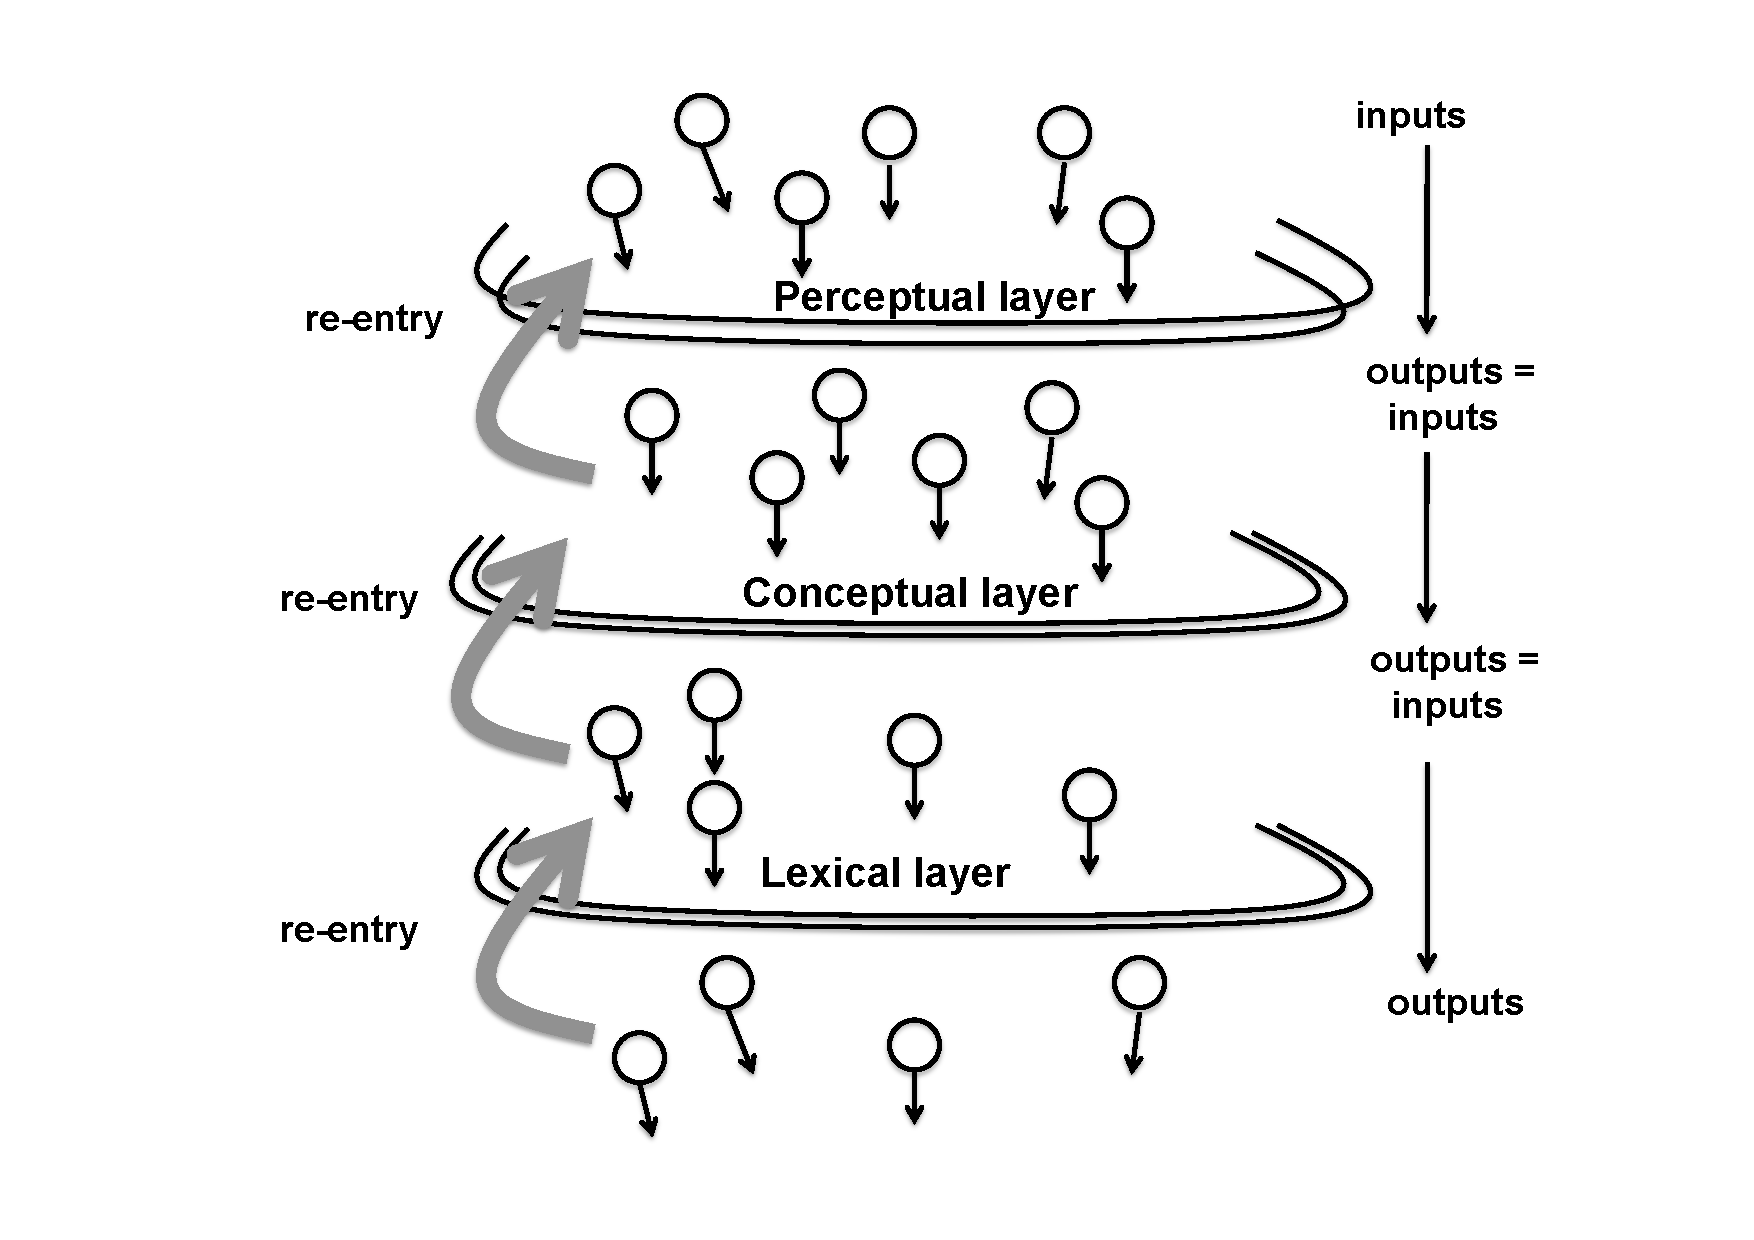
\includegraphics[width=.50\textwidth]{chap7/figs/sieve3.pdf}}
\caption{\label{sieve3}Flow of solutions through 
the different cognitive layers when an utterance is being produced.
Re-entry is necessary because the decision at each layer depends on
decisions at subsequent layers.} 
\end{figure}

For the interpretation of an utterance, the main 
flow of information goes in the other direction. The
lexical layer sends a variety of hypotheses to 
the conceptual layer and the conceptual layer makes use of data 
from the perceptual layer to see which conceptualisation
yields a referent. Several solutions are considered 
by the conceptual layer because words are typically 
ambiguous and so the perceptual 
layer must produce the appropriate segmentations and 
sensory characteristics to test each solution.
Even if a sensory channel was not considered to be 
very salient by the hearer, it may have been 
used by the speaker in his conceptualisation of the 
scene and hence the hearer's perceptual 
processes must actively try to seek in the 
image the information required to see whether it 
is applicable to the specific
context. The interpretation of an utterance
thus strongly takes the real world context into account. 
The utterance literally influences the way the 
hearer sees the world. The two-way flow (from perception
to conceptualisation and language and from language
and conceptualisation to perception) resolves one of the 
paradoxes of meaning discussed in Chapter 4. The 
clear picture of reality that we consciously experience
results from a dynamical process in which local constraints 
keep propagating until a globally coherent solution
emerges.\footnote{Dynamical systems which enter into an attractor
based on a similar relaxation process have been 
widely studied, particularly in physics. One of the 
prototypical examples is a spin glass whose magnetic
states keep switching until a globally coherent
state is reached.}

Grounding language games in the real world
not only requires a link between conceptualisation
and real world perception. Of equal importance is the physical
actions undertaken by the agents to point to the object they 
believe to be the topic. The accuracy of pointing
heavily influences overall communicative success. Indeed, a
game may fail not because
the speaker and the hearer did not agree on the meaning
nor because they did not refer to the same object, but because the 
speaker misperceived which object the hearer has pointed to. 
These differences in perception leading to difficulties
in communication do happen and may 
cause communicative failures despite a shared lexicon. 

\subsection{Concept acquisition}

I now show a series of example games taken from 
an experiment in which two situated embodied agents,
{\bfshape a1} and {\bfshape a2}, play grounded language games based on 
coloured figures pasted on the white board in front
of them. The following channels are available to the agents 
in the experiments in this section: 
\textsc{hpos} (the horizontal position of the midpoint 
of the segment's bounding box), 
\textsc{vpos} (the vertical position of the midpoint of the segment's 
bounding box), \textsc{height} (the height of the bounding box), 
\textsc{width} (the width of the bounding box), \textsc{area}
(the area of the segment, calculated
by counting the number of pixels that belong to it), 
\textsc{r} (the average redness of the pixels in the segment), 
\textsc{g} (the average greenness of the pixels in the segment), 
\textsc{b} (the average blueness of the pixels in the segment). 
These ``colour'' channels are not to be confused with the 
human opponent colour channels so the distinctions 
that form of them are not directly perceivable by 
human observers.

Because there are only two agents, the 
risk of synonymy is almost non-existent. The saliency 
threshold is sufficiently low so that more than one
sensory channel might be salient and hence ambiguity
is unavoidable. 

\begin{figure}
\begin{center}
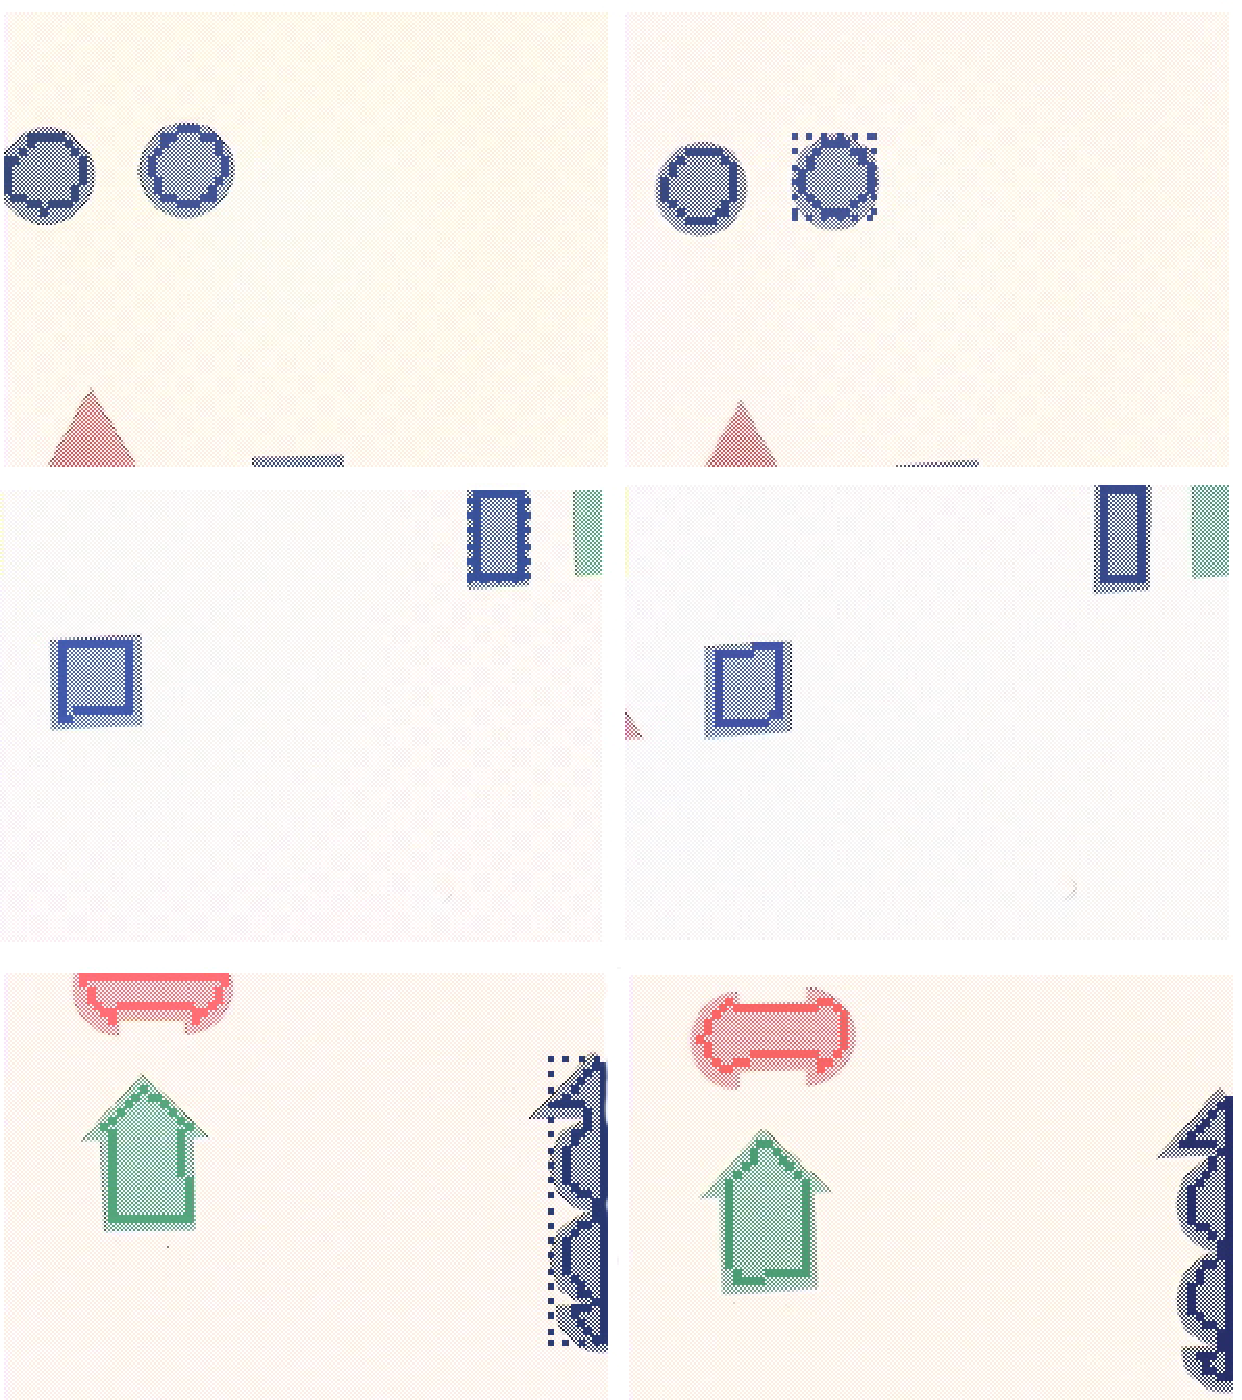
\includegraphics[width=0.8\columnwidth]{chap7/figs/plate-10.pdf}
\end{center}
\caption{Three examples of segmented images. The 
topic is indicated by a dashed bounding box in the 
image of the speaker. Segments which are too small 
are ignored. The topics have all been conceptualised
as being `to the right' and so the same word 
`gofubo' has been used to refer to them. }
\label{fig:plate-10}
\end{figure}

A first word is acquired by the agents in game 3 
based on the segmented images shown in \figref{fig:plate-10} (top).
The different sensory values (after sensor-scaling)
for the segments in game 3 are shown in \tabref{tab:game3b}. 


\begin{table}[b]
\begin{center}
\begin{tabular}{lll}
\lsptoprule
{\itshape channel}& {\itshape obj-0} & {\itshape obj-1}\\ \midrule
\textsc{hpos} & 0.27 & 0.16\\ 
\textsc{vpos} & 0.20 & 0.20\\ 
\textsc{height} & 0.15 & 0.15\\ 
\textsc{width} & 0.10 & 0.11\\ 
\textsc{area} & 0.10 & 0.10\\ 
R & 0.23 & 0.25\\ 
G & 0.32 & 0.34\\ 
B & 0.63 & 0.65\\ 
\lspbottomrule
\end{tabular}
\caption{\label{tab:game3b}First words after about a dozen games.}
\end{center}
\end{table}
\clearpage
\textsc{hpos} is the most salient channel. After sensor-scaling, 
the two values for \textsc{hpos} are still be drawn further
apart with 1.0 for object-0 and 
0.0 for object-1 so that the category [\textsc{hpos} 0.5–1.0] easily 
distinguishes the topic (object-0) from object-1.

The left image is that of the hearer {\bfshape a1}, the right one
that of the speaker, {\bfshape a2}.
{\bfshape a2} had already invented the word `gofubo' for 
[\textsc{hpos} 0.5–1.0] (to the right) in an earlier game, 
but the word was not acquired in that game
by {\bfshape a1} because he still missed the 
appropriate distinction. Meanwhile the \textsc{hpos} category 
is available to {\bfshape a1} due to an
expansion of his discrimination networks
and so he can store the word: 
\begin{verbatim}
Game 3 
  a2 is the speaker. a1 is the hearer. 
  a2 segments the context into 2 objects: 
       object-0 object-1
  a2 chooses object-0 as the topic 
  a2 categorises the topic as [\textsc{hpos} 0.5–1.0]
  a2 says: gofubo
  a1 does not know gofubo
  a1 says: gofubo?
  a2 points to object-0
  a1 categorises the topic as [\textsc{hpos} 0.5–1.0]
  a1 stores gofubo as [\textsc{hpos} 0.5–1.0]
\end{verbatim}
This game proceeds essentially like in the computer
simulations studied before. The major difference is
that now real images have been used, the objects
considered are the outcome of segmentation processes,
the sensory characteristics have been derived from the 
image itself, and the pointing has been done by 
physically moving the cameras. 

\subsection{Generalisation without learning}

Immediately the agents apply this word to very 
different scenes, such as the ones in \figref{fig:plate-10} (middle and bottom). The middle picture
shows on the left the segmented scene
from the speaker in game 5, and on the right the one
from the hearer. In game 5, the figures are blue
rectangles. They are much further apart than 
the two circles in game 3. Nevertheless, 
after scaling, they are categorised and
conceptualised similarly and therefore
the same word could be used effectively. The concept 
of [\textsc{hpos} 0.5–1.0] and hence the word `gofubo' 
is general {\itshape from the very start}. 
The agents do not need to see many examples because they do 
not use inductive generalisation. Instead, 
the \textsc{hpos} category is constructed in a top-down fashion 
as soon as the \textsc{hpos} channel has been salient
and is immediately available for use in the 
discrimination game and hence in verbalising 
the scene. This explains why the word-meaning acquisition
process observed in the experiments goes so 
amazingly fast.

The bottom of \figref{fig:plate-10}
shows yet another scene where the word `gofubo' 
was used with success. The topic is the rightmost
shape in the scene and so [\textsc{hpos} 0.5–1.0] is once more 
distinctive. To an outside observer it may look 
like the agents have performed a gigantic inductive
leap, but this is not the case at all. The agents
do not try to abstract the commonalities from 
different examples but construct distinctions in a top 
down fashion and try to apply them to the perceived image. 

After a mere 50 games, the lexicon shown in \tabref{tab:game50} has emerged. Only
associations with scores greater than 0.0 are shown. 

\begin{table}
\begin{center}
\begin{tabular}{lllll}
\lsptoprule
{\itshape Word}&{\itshape Meaning}&{\itshape Translation} & {\bfshape a1}&{\bfshape a2} \\ \midrule
wawosido & [\textsc{hpos} 0.0–0.5] &left&0.4&0.4\\ 
meluri & [\textsc{hpos} 0.25–0.5] &medium left&0.1&0.0\\ 
gofubo & [\textsc{hpos} 0.5–1.0]& right&1.0&1.0\\ 
wiwigapo & [\textsc{vpos} 0.0–0.5] &left&0.1&0.0\\ 
fozumoba & [\textsc{area} 0.5–1.0]&large & 0.0&0.1\\ 
wefoto & [\textsc{r} 0.0–0.5]& low redness &0.2&0.2\\ 
togene & [\textsc{r} 0.5–1.0]& high redness &0.5&1.0\\ 
fumudanu & [\textsc{g} 0.0–0.5]& low greenness &0.2&0.2\\ 
puxedu & [\textsc{g} 0.5–1.0]& high greenness &0.4&0.4\\ 
\lspbottomrule
\end{tabular}
\caption{\label{tab:game50}First words after about a dozen games.}
\end{center}
\end{table}

There is already a word (`gofubo') which has
a score of 1.0! After 100 games, the lexicon has become more 
solid and now looks as in \tabref{tab:goubo}.    


\begin{table}
\begin{center}
\begin{tabular}{lllll}
\lsptoprule
{\itshape Word}&{\itshape Meaning}&{\itshape Translation} & {\bfshape a1}&{\bfshape a2} \\ \midrule
wawosido & [\textsc{hpos} 0.0–0.5] &left&0.7&0.5\\ 
meluri & [\textsc{hpos} 0.25–0.5] &medium left&0.4&0.4\\ 
gofubo & [\textsc{hpos} 0.5–1.0]& right&1.0&1.0\\ 
vokomutu & [\textsc{hpos} 0.5–0.75] &medium right&0.2&0.2\\ 
buwonipo & [\textsc{hpos} 0.75–0.875] &strongly right&0.1&0.0\\ 
wiwigapo & [\textsc{vpos} 0.0–0.5] &down&0.6&0.6\\ 
fozumoba & [\textsc{area} 0.5–1.0]&large & 0.2&0.4\\ 
wefoto & [\textsc{r} 0.0–0.5]& low redness &0.2&0.3\\ 
togene & [\textsc{r} 0.5–1.0]& high redness &1.0&1.0\\ 
fumudanu & [\textsc{g} 0.0–0.5]& low greenness &0.7&0.7\\ 
puxedu & [\textsc{g} 0.5–1.0]& high greenness &0.7&0.9\\ 
\lspbottomrule
\end{tabular}
\caption{\label{tab:goubo}Population lexicon after 100 games.}
\end{center}
\end{table}


\begin{figure}[htbp]
  \centerline{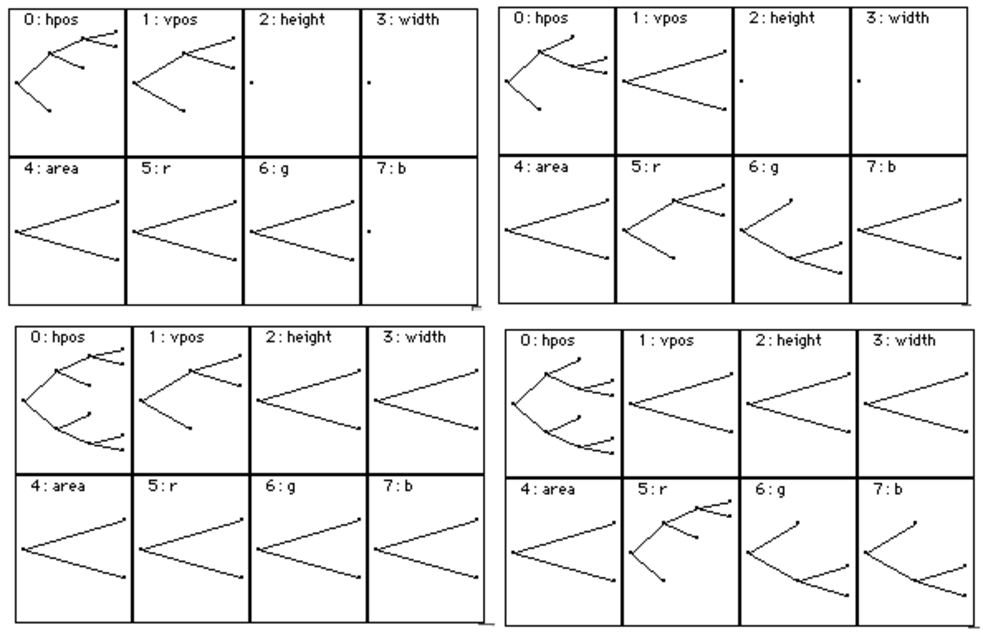
\includegraphics[width=.75\textwidth]{chap7/figs/discri200.pdf}}
\caption{\label{discri200}The discrimination trees 
of two embodied agents {\bfshape a1} (left) and {\bfshape a2} (right) 
after playing 100 games (top) and after 200 games (bottom).}
\end{figure}

\subsection{The influence of the environment}

One thing is striking about this lexicon. It contains\is{environmental influence}
words for fine-grained distinctions along the 
horizontal position axis, but none for width or 
height. Indeed if we look at the discrimination
trees as they exist at this point (figure 
\ref{discri200} top) we see that there are no 
discrimination trees for the \textsc{height} and \textsc{width}
channels. This is entirely due to the 
environment. There have simply been no situations on 
the white board yet where these distinctions are salient 
enough. 

As human experimenters, we can stimulate conceptual 
development by configuring scenes where these
channels are needed, for example, a scene 
which contains two objects with the same size, colour, 
and position but of significantly different width. The 
conceptual layer in each agent
should then start to develop again
and the lexical layer should follow with the 
construction of new words. 


\begin{figure}
\begin{center}
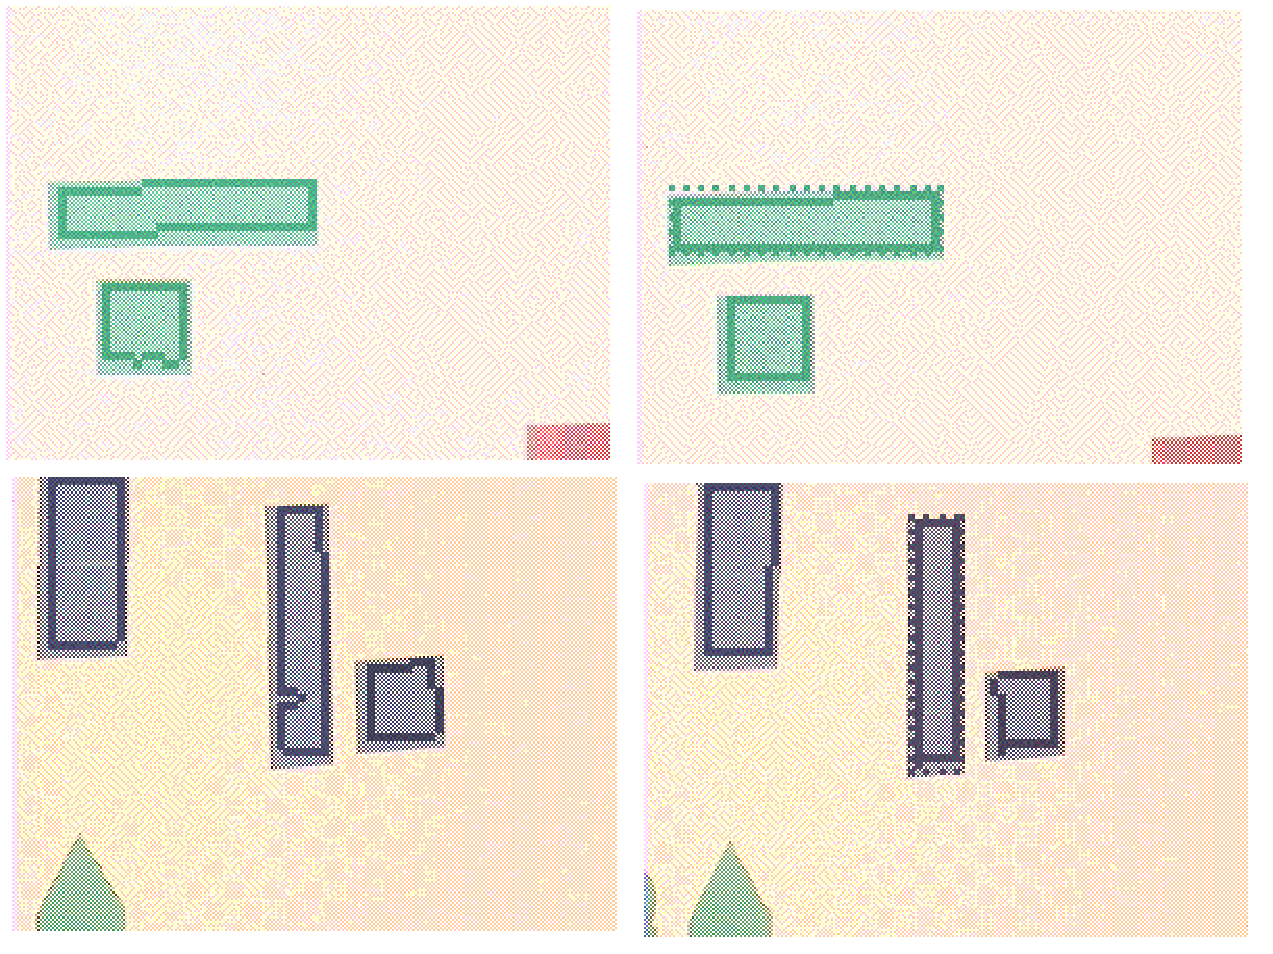
\includegraphics[width=0.8\columnwidth]{chap7/figs/plate-13.pdf}
\end{center}
\caption{Top and bottom: Examples of new segmented scenes that stimulate conceptual development
and hence expansions of the lexicon. The most salient characteristic in the top scene is \textsc{width} and in the bottom 
scene \textsc{height}.}
\label{fig:plate-13}
\end{figure}

A game where this happens is game 126 with the segmented images
shown in \figref{fig:plate-13} (top). Width is now the most salient
channel. The segments and sensory data for game 126 
(after sensor-scaling) are shown in \tabref{tab:game126}. 

\begin{table}
\begin{center}
\begin{tabular}{lll}
\lsptoprule
{\itshape channel}& {\itshape obj-0} & {\itshape obj-1}\\ \midrule
\textsc{hpos} & 0.08 & 0.09\\ 
\textsc{vpos} & 0.21 & 0.10\\ 
\textsc{height} & 0.10 & 0.15\\ 
\textsc{width} & 0.42 & 0.11\\ 
\textsc{area} & 0.34 & 0.16\\ 
\textsc{r} & 0.33 & 0.31\\ 
\textsc{g} & 0.68 & 0.65\\ 
\textsc{b} & 0.52 & 0.50\\ 
\lspbottomrule
\end{tabular}
\caption{\label{tab:game126}Sensory data for game 126.}
\end{center}
\end{table}
Clearly width is the most salient channel for the speaker. 
It is therefore chosen and because the 
agents have already grown distinctions on this channel, 
discrimination succeeds and a new word can be
constructed and stored. 
\begin{verbatim}
Game 126 
  a2 is the speaker. a1 is the hearer. 
  a2 segments the context into 2 objects: 
       object-0 object-1
  a2 chooses object-0 as the topic 
  a2 categorises the topic as [\textsc{width} 0.5–1.0]
  a2 creates a new word: vaviwumu
  a2 says: vaviwumu
  a1 does not know vaviwumu
  a1 says: vaviwumu?
  a2 points to object-0
  a1 categorises the topic as [\textsc{width} 0.5–1.0]
  a1 stores vaviwumu as [\textsc{width} 0.5–1.0]
\end{verbatim}
\figref{fig:plate-13} (bottom) contains another example
of segmented images which have stimulated conceptual
growth and hence an expansion of the lexicon. 
In this case, categorisations on the \textsc{height} channel are
relevant and a word developed for tall.

\begin{figure}
\begin{center}
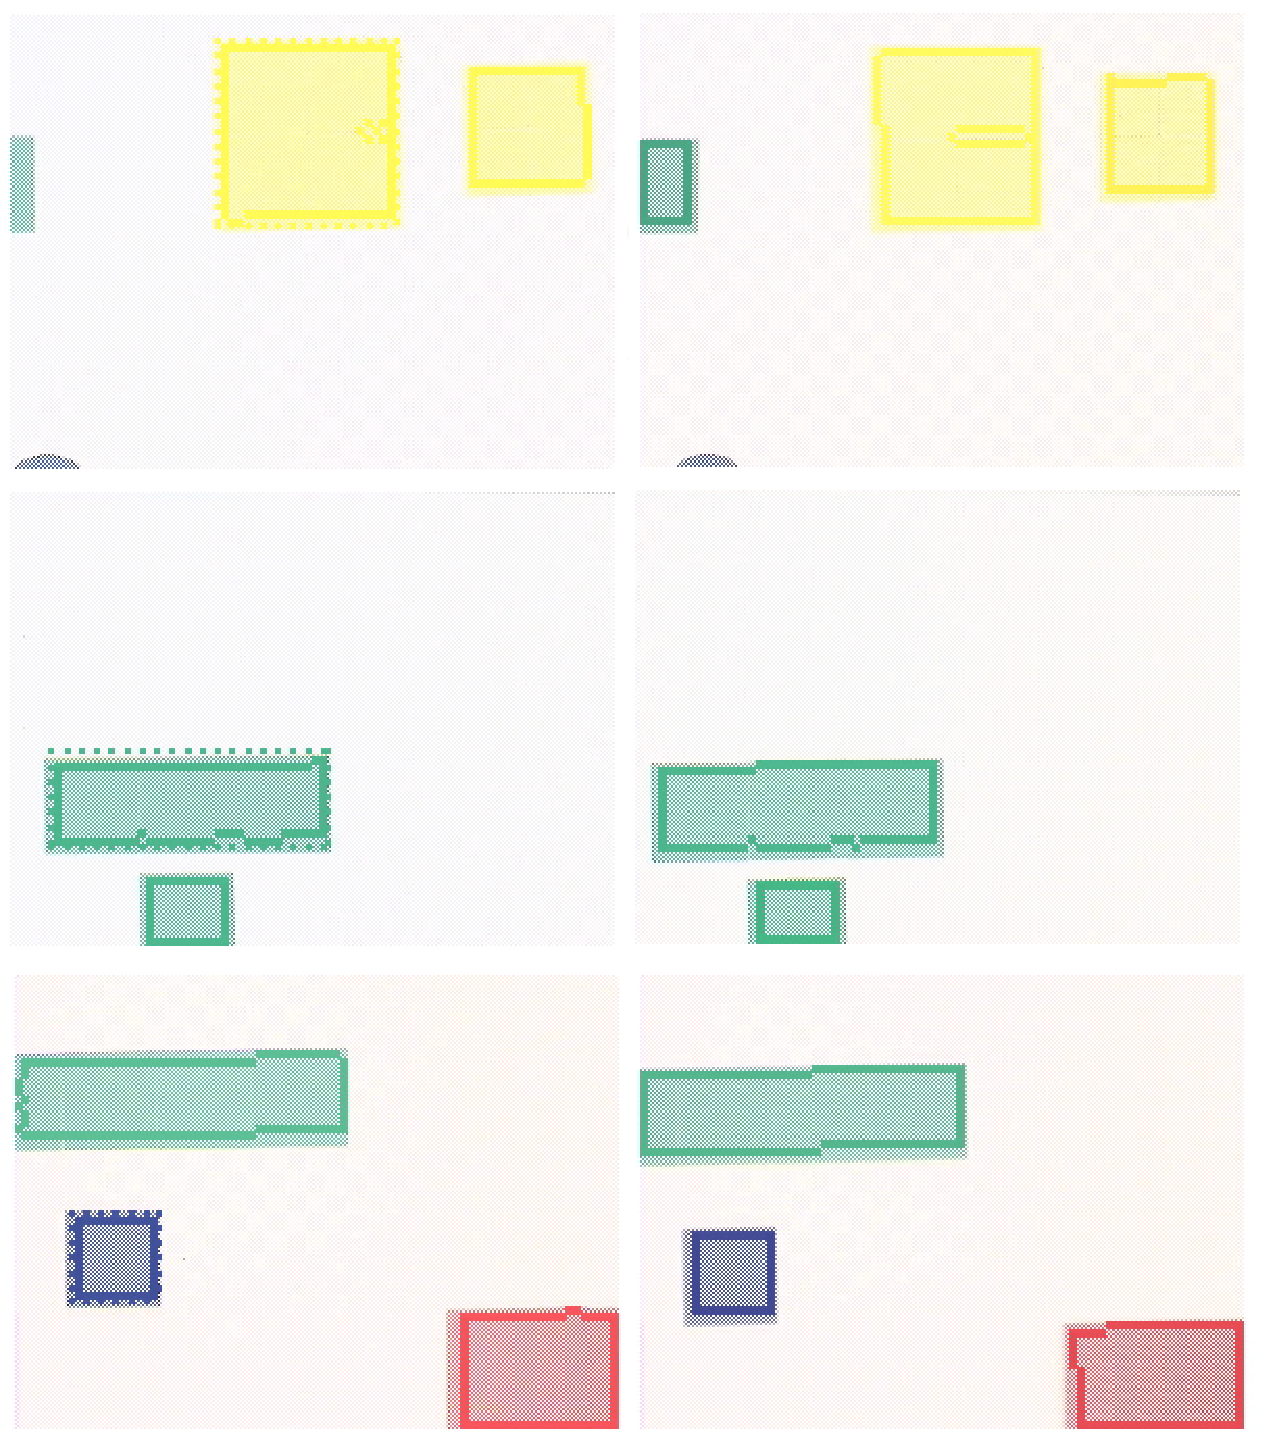
\includegraphics[width=0.8\columnwidth]{chap7/figs/plate-14-area.pdf}
\end{center}
\caption{Segmented images where distinctions on the \textsc{area} channel have been used. The topic (with dashed bounding 
box) in the two top cases has been categorised as large. In the bottom case, a word meaning `small' was used.}
\label{fig:plate-14}
\end{figure}

\figref{fig:plate-14} shows another series of image segments, 
where categorisations based on the \textsc{area} channel were effective
and \figref{fig:plate-15} shows additional image segments exercising
\textsc{vpos}, \textsc{hpos} and colour distinctions. 

\begin{figure}
\begin{center}
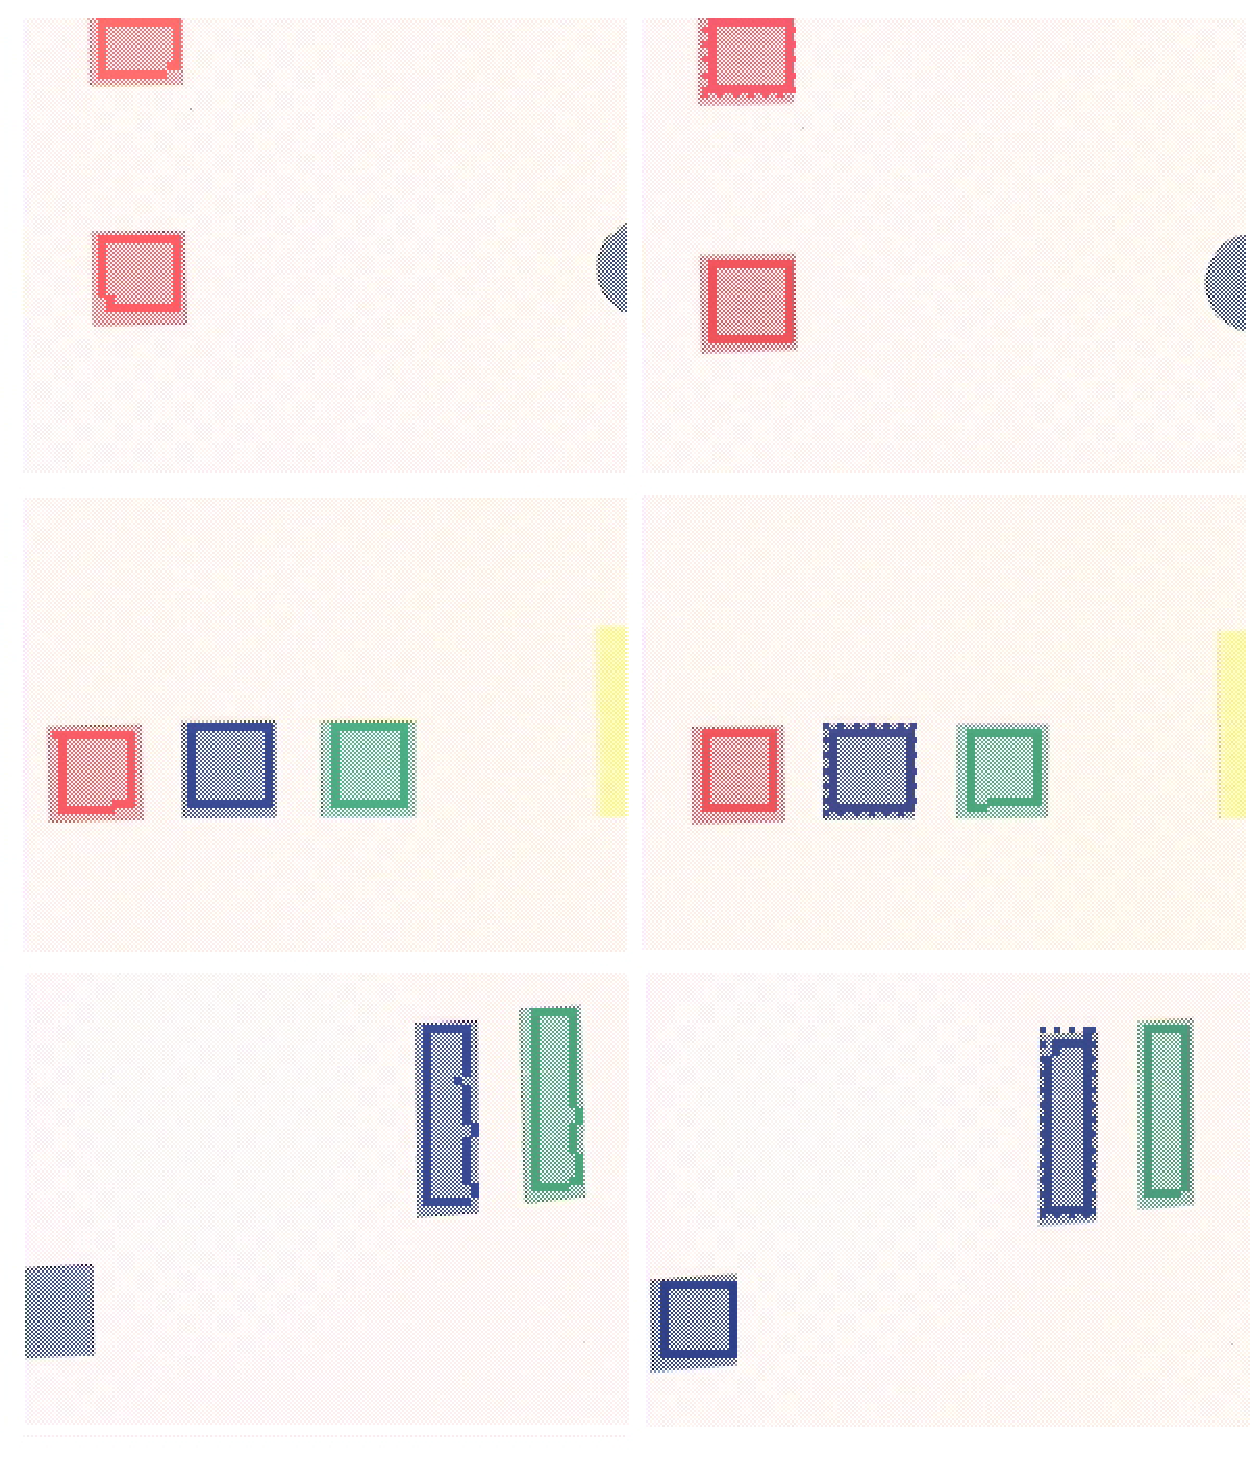
\includegraphics[width=0.8\columnwidth]{chap7/figs/plate-15-vpos.pdf}
\end{center}
\caption{The image segments from the top game require 
distinctions on the \textsc{vpos} channel and 
caused the creation of a word for `upper'. The image 
segments in the middle lead to the use of refined
distinctions on the \textsc{hpos} channel, so as to 
identify the middle square. The topic in the 
image segments at the bottom was done with a 
conjunction of categories: blue and tall.}
\label{fig:plate-15}
\end{figure}

After 200 games, the lexicon of the population looks as in \tabref{tab:upper}. 

\begin{table}
\begin{center}
\begin{tabular}{lllll}
\lsptoprule
{\itshape Word}&{\itshape Meaning}&{\itshape Translation} & {\bfshape a1}&{\bfshape a2} \\ \midrule
wawosido & [\textsc{hpos} 0.0–0.5] &left&0.9&0.4\\ 
gixepo & [\textsc{hpos} 0.0–0.25] & very left&0.4&0.4\\ 
wonuxa & [\textsc{hpos} 0.0–0.25] & very left&0.10&0.0\\ 
meluri & [\textsc{hpos} 0.25–0.5] &medium left&0.4&0.4\\ 
gofubo & [\textsc{hpos} 0.5–1.0]& right&1.0&1.0\\ 
vokomutu & [\textsc{hpos} 0.5–0.75] &medium right&0.4&0.4\\ 
buwonipo & [\textsc{hpos} 0.75–0.875] &strongly right&0.1&0.0\\ 
wiwigapo & [\textsc{vpos} 0.0–0.5] &down&0.5&0.4\\ 
putuwenu & [\textsc{vpos} 0.5–1.0]&up & 0.5&0.5\\ 
vaviwumu & [\textsc{width} 0.5–1.0]&wide & 0.5&0.5\\ 
pesidumu & [\textsc{area} 0.0–0.5]&small& 0.2&0.2\\ 
fozumoba & [\textsc{area} 0.5–1.0]&large & 1.0&1.0\\ 
wefoto & [\textsc{r} 0.0–0.5]& low redness &0.2&0.1\\ 
togene & [\textsc{r} 0.5–1.0]& high redness &0.9&1.0\\ 
fumudanu & [\textsc{g} 0.0–0.5]& low greenness &0.7&0.9\\ 
puxedu & [\textsc{g} 0.5–1.0]& high greenness &0.9&0.9\\ 
\lspbottomrule
\end{tabular}
\caption{\label{tab:upper}Population lexicon after 200 games.}
\end{center}
\end{table}
Note that new words have come into the lexicon 
for up (`putuwenu'), down (`wiwigapo'), and 
wide (`vaviwumu'). The discrimination trees of 
the \textsc{width} and \textsc{height} channel have started to 
expand (\figref{discri200} bottom). 

\subsection{Coping with perceptual anomalies}

Grounding language games in physical environments\is{perceptual anomalies}
makes it obviously harder
for the agents in a number of respects. First of 
all because perception and segmentation may differ, 
the salient characteristics of objects may not be the same
and as a result the hearer may guess another meaning for an 
unknown word, compared to 
the one used by the speaker. This happens for
example in the following game (game 128) which is based on 
the segmented images shown in \figref{fig:plate-16} (top). The
speaker's perception is shown to the left and the 
hearer's to the right. 
\begin{verbatim}
Game 128
  a1 is the speaker. a2 is the hearer. 
  a1 segments the context into 3 objects: 
       object-0 object-1 object-2
  a1 chooses object-0 as the topic 
  a1 categorises the topic as 
       [HPOS 0.0–0.25] [HPOS 0.0–0.125]
  a1 creates a new word: `bagaxe' for [HPOS 0.0–0.25]
  a1 says: bagaxe
  a2 does not know bagaxe
  a2 says: bagaxe?
  a1 points to object-0
  a2 categorises the topic as [AREA 0.5–1.0]
  a2 stores bagaxe as [AREA 0.5–1.0]
\end{verbatim}


\begin{figure}
\begin{center}
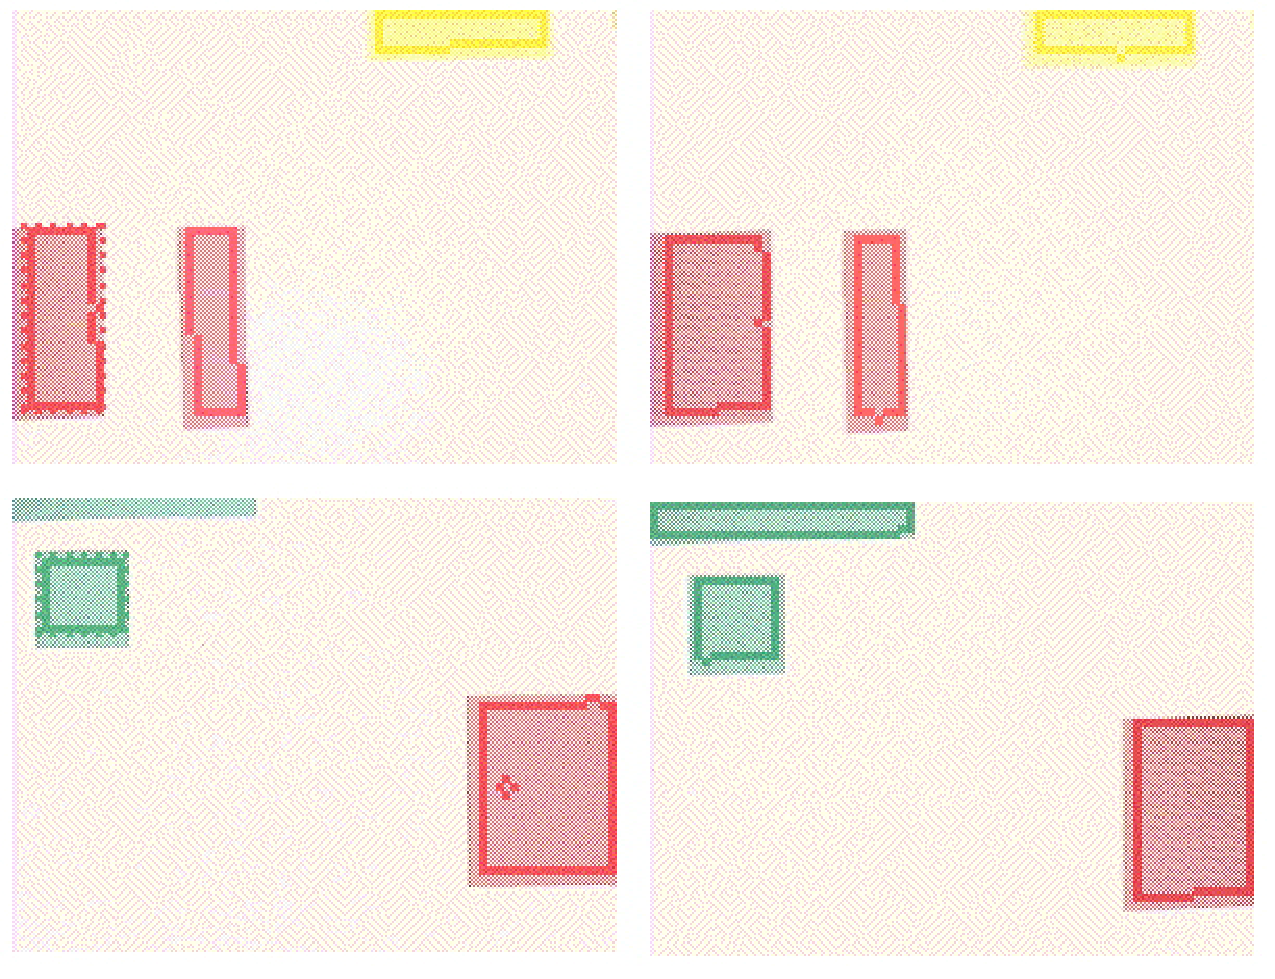
\includegraphics[width=0.8\columnwidth]{chap7/figs/plate-16.pdf}
\end{center}
\caption{Examples of scenes causing confusion
due to perceptual anomalies. In the top scene, 
the segmentation of the speaker (left) makes the 
topic's most salient characteristic the horizontal
position, whereas for the hearer (right) the most salient
characteristic of the same segment is its area. In the 
bottom scene, speaker and hearer have segmented the 
scene into two, respectively three segments. This 
causes the game to fail even though both agents 
had the same meaning for the word used by the speaker.}
\label{fig:plate-16}
\end{figure}

Although the difference may not appear significant to 
the human eye, the topic (the left most rectangle) is 
in the raw perception of the speaker less wide as the same 
rectangle perceived by the hearer. 
The segments and sensory data of the speaker
in game 128 (after sensor-scaling) are shown in the 
\tabref{tab:game128}. 

\begin{table}
\begin{center}
\begin{tabular}{llll}
\lsptoprule
{\itshape channel}& {\itshape obj-0} & {\itshape obj-1} & {\itshape obj-2}\\ 
\textsc{hpos} & 0.03 & 0.15 & 0.33\\ 
\textsc{vpos} & 0.29 & 0.29 & 0.01\\ 
\textsc{height} & 0.37 & 0.39 & 0.07\\ 
\textsc{width} & 0.10 & 0.08 & 0.27\\ 
\textsc{area} & 0.29 & 0.22 & 0.16\\ 
R & 0.95 & 0.97 & 0.97 \\ 
G & 0.33 & 0.40 & 0.93\\ 
B & 0.35 & 0.44 & 0.26\\ 
\lspbottomrule
\end{tabular}
\caption{\label{tab:game128}Sensory data for game 128.}
\end{center}
\end{table}
Context-scaling further
amplifies this difference which shows that it is not 
always beneficial to do so. {\bfshape a1} uses
the horizontal axis, creating a new word `bagaxe' 
meaning `very left' [\textsc{hpos} 0.0–0.25] whereas {\bfshape a2}, for
whom the area is the most salient characteristic, 
associates this word with [\textsc{area} 0.5–1.0] (large). 
This example shows that grounding introduces 
additional risks for the introduction of semantic
incoherence in a group's lexicon. 

Due to perceptual anomalies, a game may fail even though 
both agents already have the same meaning for the 
same word. This happens when this meaning yields different 
objects (or no objects at all) for the speaker and the hearer. 
As a consequence, the hearer adopts another meaning for 
the word which starts to compete with the one he already had. 
This happened in the following game (game 127)
based on the segmented images shown in \figref{fig:plate-16} (bottom). The speaker (left image) has identified
only two objects, but the hearer three. The 
speaker (left image) uses green as distinguishing 
characteristic which is indeed appropriate. but 
because the hearer's third object (the top rectangle) is 
also green, this distinction fails for him.  
Even though the hearer had already a well established
meaning for `puxedu', he associates a new meaning 
based on the \textsc{width}-channel with this word because this 
channel is now the most salient. 
\begin{verbatim}
Game 127
  a1 is the speaker. a2 is the hearer. 
  a1 segments the context into 2 objects: 
       s-object-0 s-object-1
  a1 chooses object-0 as the topic 
  a1 considers as salient G R AREA HPOS 
  a1 categorises the topic as 
       [HPOS 0.0–0.5] [HPOS 0.0–0.125]
       [AREA 0.0–0.5] [R 0.0–0.5] [G 0.5–1.0]
  a1 has the words
       puxedu for [G 0.5–1.0] (1.0)
       wawosido for [HPOS 0.0–0.5] (0.7)
       pesidimu for [AREA 0.0–0.5] (0.2)
       wefoto for [R 0.0–0.5] (0.2)
       buwonipo for [G 0.5–1.0] (0.0)
  a1 says: puxedu
  a2 segments the context into 3 objects: 
       h-object-0 h-object-1 h-object-2
  a2 interprets puxedu as
       [G 0.5–1.0] (0.20)
  a2 identifies h-object-0 h-object-1
  a2 says: puxedu?
  a1 points to s-object-0
  a2 categorises the topic as [WIDTH 0.5–1.0]
  a2 stores puxedu as [WIDTH 0.5–1.0]
\end{verbatim}

After 500 games, the lexicon is as in \tabref{tab:puxedu}. 

\begin{table}
\begin{center}
\begin{tabular}{lllll}
\lsptoprule
{\itshape Word}&{\itshape Meaning}&{\itshape Translation} & {\bfshape a1}&{\bfshape a2} \\ \midrule
wawosido & [\textsc{hpos} 0.0–0.5] &left&0.9&0.4\\ 
gixepo & [\textsc{hpos} 0.0–0.25] & very left&0.4&0.4\\ 
wonuxa & [\textsc{hpos} 0.0–0.25] & very left&0.10&0.0\\ 
meluri & [\textsc{hpos} 0.25–0.5] &medium left&0.4&0.4\\ 
gofubo & [\textsc{hpos} 0.5–1.0]& right&1.0&1.0\\ 
vokomutu & [\textsc{hpos} 0.5–0.75] &medium right&0.4&0.4\\ 
buwonipo & [\textsc{hpos} 0.75–0.875] &strongly right&0.1&0.0\\ 
wiwigapo & [\textsc{vpos} 0.0–0.5] &down&0.5&0.4\\ 
putuwenu & [\textsc{vpos} 0.5–1.0]&up & 0.5&0.5\\ 
vaviwumu & [\textsc{width} 0.5–1.0]&wide & 0.5&0.5\\ 
pesidumu & [\textsc{area} 0.0–0.5]&small& 0.2&0.2\\ 
fozumoba & [\textsc{area} 0.5–1.0]&large & 1.0&1.0\\ 
wefoto & [\textsc{r} 0.0–0.5]& low redness &0.2&0.1\\ 
togene & [\textsc{r} 0.5–1.0]& high redness &0.9&1.0\\ 
fumudanu & [\textsc{g} 0.0–0.5]& low greenness &0.7&0.9\\ 
puxedu & [\textsc{g} 0.5–1.0]& high greenness &0.9&0.9\\ 
\lspbottomrule
\end{tabular}
\caption{\label{tab:puxedu}Population lexicon after 500 games.}
\end{center}
\end{table}
The global evolution of success and ontology is shown in the 
graph in \figref{psuccess1}. The graph is not 
fundamentally different from the ones we have
seen in the computer simulations in the previous
chapter, except that more failures occur after a lexicon
is established due to the contingencies of real 
world images and the unavoidable stochasticity 
associated with physical interactions. 

\begin{figure}[htbp]
  \centerline{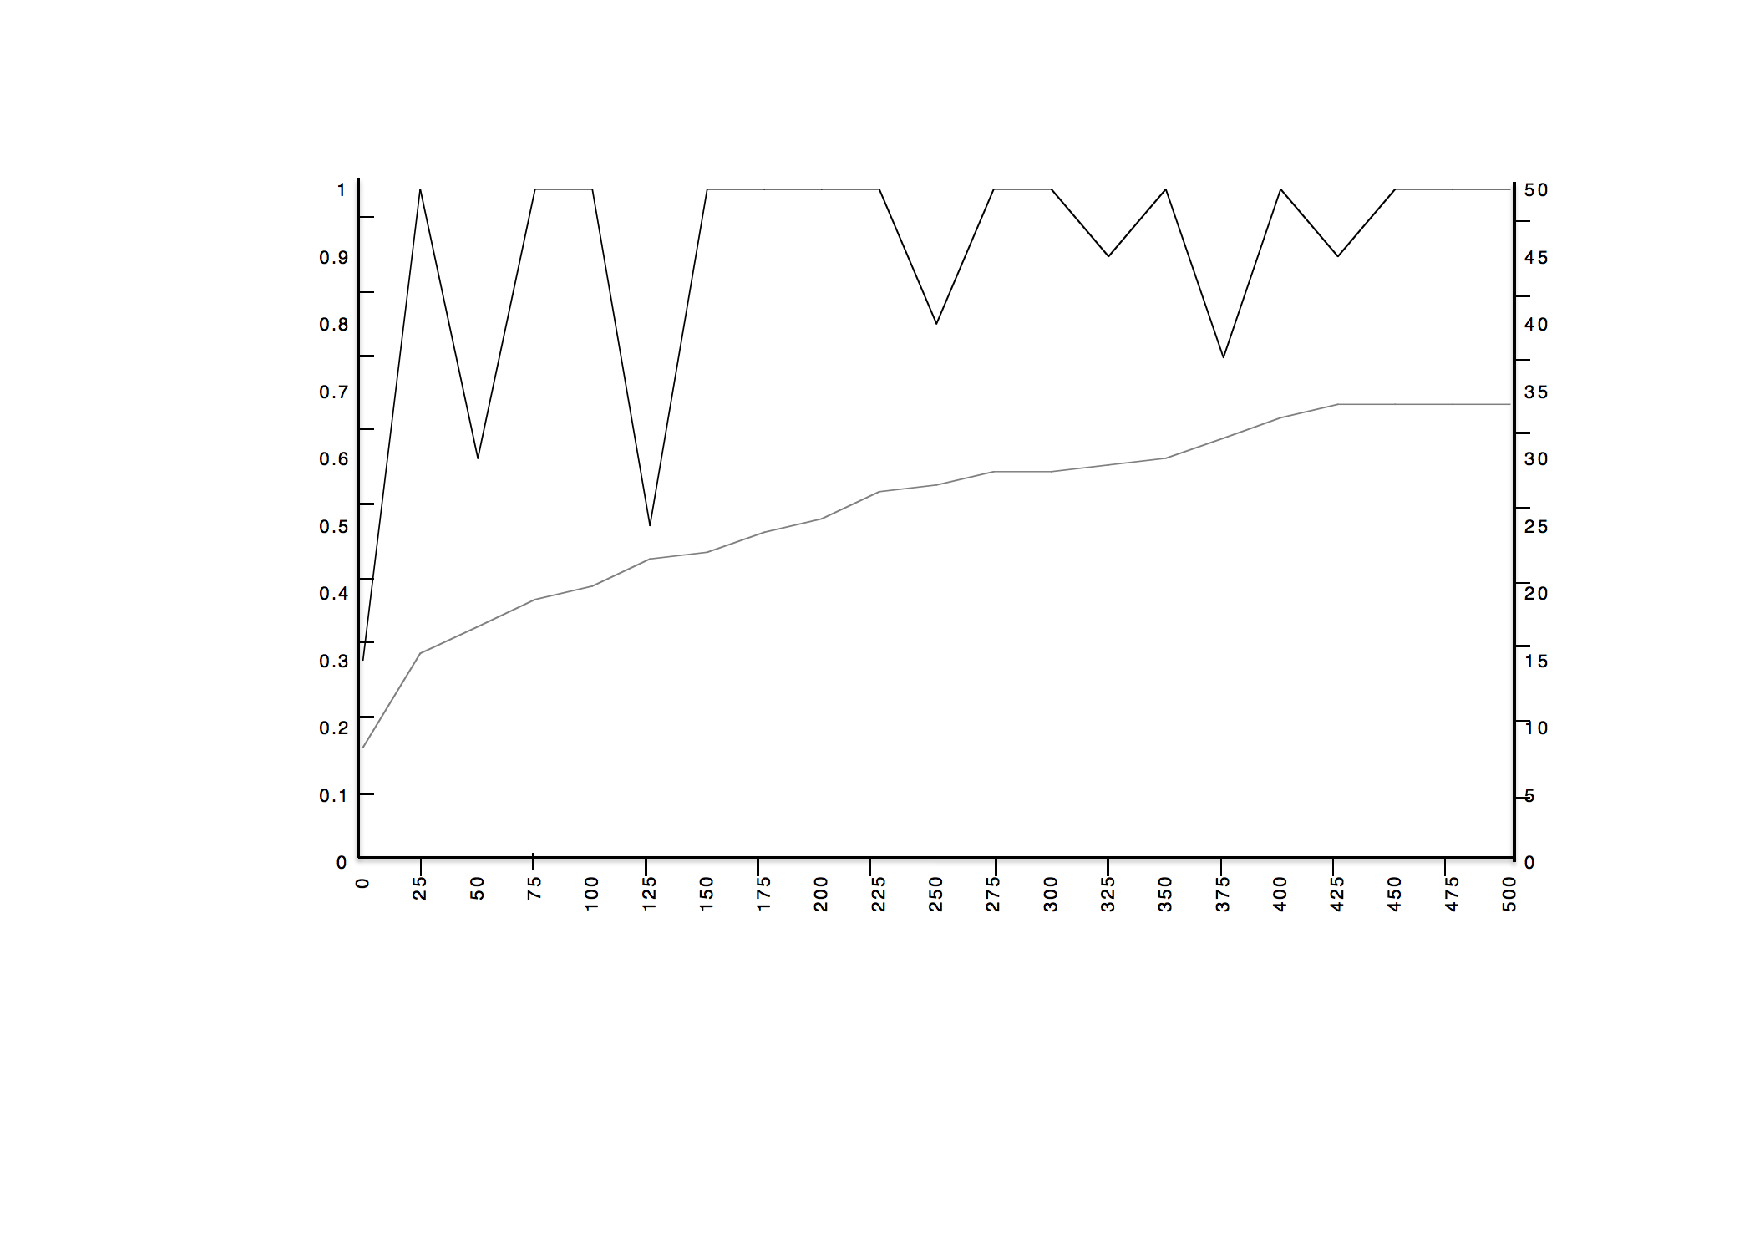
\includegraphics[width=.70\textwidth]{chap7/figs/psucc500.pdf}}
\caption{\label{psuccess1}Success 
(left y-axis) and average ontology size
(right y-axis) for two agents playing 500
guessing games about real world scenes perceived
through their cameras. Occasionally new situations
have been introduced to stimulate conceptual development.} 
\end{figure}

So despite the difficulties caused by perceptual anomalies
and errors in non-verbal real-world interaction, the 
mechanisms used by the agents appear sufficiently 
robust that a shared communication system manages to get 
off the ground. We have been able to 
take away all the scaffolds put up in earlier
chapters and the complete language system now stands on its own
feet. Of course we now need to further scale up the 
challenge to the agents, particularly along three
dimensions: complexity of the environments, complexity 
of the sensori-motor apparatus (particularly the number of
sensory channels available to the agents), and
size of the agent population. Only the latter type of 
scale-up is studied in the remainder of this chapter. 

\section{Semiotic dynamics} 

Semiotic dynamics refers to the changing relationships\is{semiotic dynamics}
between words, meanings, perceptions,
and real world scenes observed while a group of
autonomous distributed agents play language games
about scenes from an open evolving environment. 
The possible utterances and
possible meanings are not fixed but continuously
changing as the agents autonomously evolve their
communication systems and adapt to changing
environments. Tracking and understanding these
changes is a non-trivial task. It is comparable to 
the investigation of other non-linear complex dynamical
systems and therefore similar tools are useful.\footnote{
See \cite{Badii:1997}. 
Examples of ways to model evolutionary systems are shown in 
\cite{Kauffman:1993} and \cite{Maynard:1989}.}
The study of semiotic dynamics is an entirely new subject
for linguistics, and I will give here only some
examples to illustrate the approach. 

\subsection{Tracking language evolution}

The first thing we need is a systematic
way to collect data. In studying the lexical 
and ontological development 
of the agents, I have so far played god, inspecting 
the internal states of the agents. With larger agent
populations that 
are travelling over the Internet and engage in interactions in 
different physical sites, it becomes impossible
to perform these computations, because ontologies and 
lexicons are distributed over many agent servers
throughout the world and different language games are
going on in parallel. We 
are forced in these circumstances to adopt the
viewpoint of a linguist, who
can only observe the overt linguistic behavior in the community,
not the internal states of each individual. 
So we have built tools that track the language games 
as they take place in parallel on a world-wide scale. The tools 
are available to anyone who logs on through the Internet
and wants to see for him or herself how the language
system is evolving.\footnote{The website http://talking-heads.csl.sony.fr/ 
contains the latest statistics on this world-wide evolution. 
The observational tools were mainly built by Joris Van 
Looveren and Frederic Kaplan.}

Of course, an external observer's
point of view is only partial. As we have seen in the
previous chapters, many 
words and categories are latently known by the agents, 
without their being used in overt behavior, just as 
we carry genes in our bodies that are not 
being expressed. Nevertheless, 
observations of the actual behavior of the agents is
in a sense a more natural way to characterise 
ontologies and lexicons and reflects well the
semiotic dynamics in the population. For the remainder
of this chapter, all data
are taken from observing experiments with the Talking Heads as
they play grounded language games. 

\subsection{Semiotic landscapes}

A semiotic landscape contains all the semiotic relationships\is{semiotic landscape}
that effectively occurred at least once
in the games played by a particular population of agents
during a certain period of time. 
The semiotic landscape is a graph. The nodes in the
graph are formed by situations (referents in a specific context), 
meanings, and forms (words),
and there are links if the items associated with two nodes
indeed co-occur (\figref{RMF1}). In a more complete
picture, the landscape makes a distinction between 
external referents and segmented images but I will not 
do so in the present chapter. The relations in the landscape are labeled as in \tabref{tab:7labelrelation}.

\begin{figure}[htbp]
  \centerline{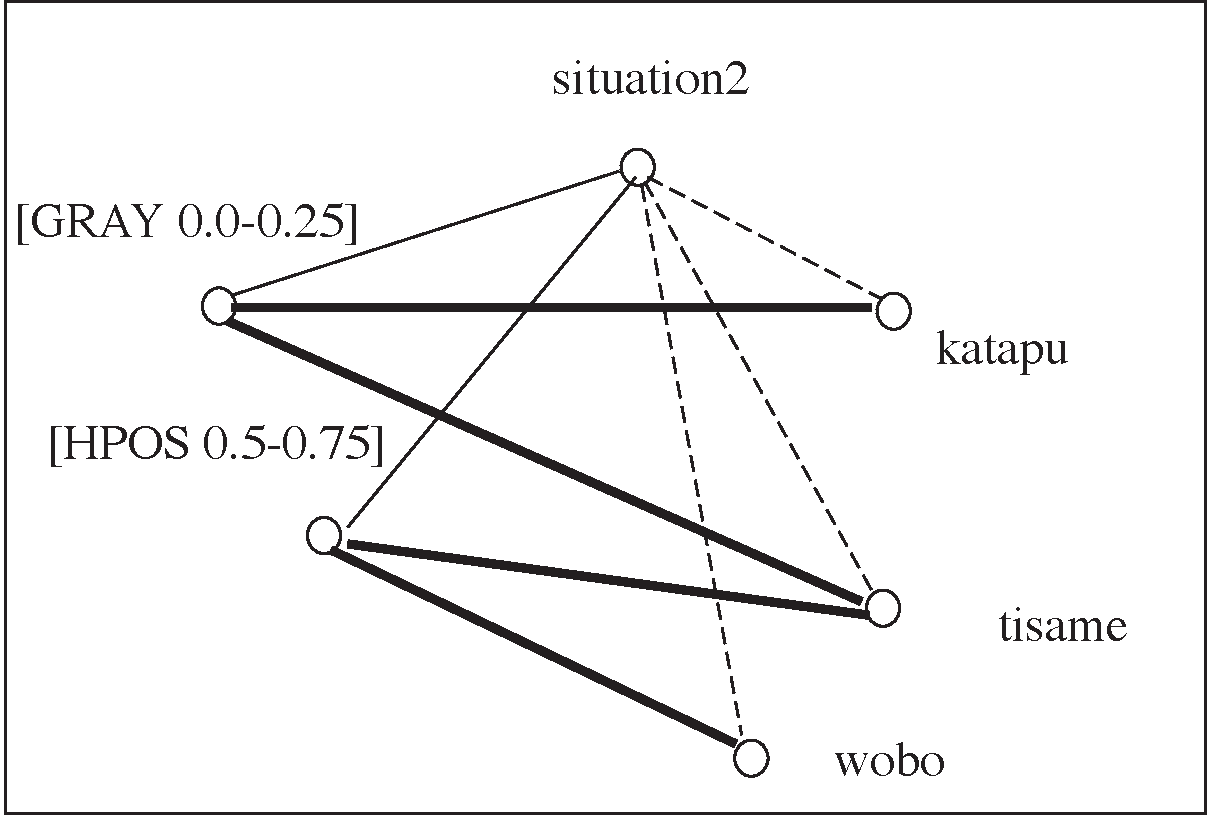
\includegraphics[width=.65\textwidth]{chap7/figs/landscape.pdf}}
\caption{\label{RMF1}Typical segment of a semiotic
landscape capturing the co-occurrence relations between
referents, meanings and word forms. The FM/MF relations are
in thick lines, the RM/MR relations in regular lines, and 
the RF/FR relations in dashed lines.}
\end{figure}
 
\begin{center}
\begin{table}
\begin{tabular}{ l  l  }
\lsptoprule
{\itshape Label}& {\itshape Relation } \\ \midrule
RM & referent to meaning \\ 
MR & meaning to referent \\ 
FM & form to meaning\\ 
MF & meaning to form\\ 
RF & referent to form \\ 
FR & form to referent  \\ 
\lspbottomrule
\end{tabular}
\caption{\label{tab:7labelrelation}}
\end{table}
\end{center}

The partial landscape in \figref{RMF1} (taken from
an actual experiment) contains an example where the agents use
two possible meanings for conceptualising {\itshape situation2}, namely
[\textsc{gray} 0.0–0.25] (very light) and [\textsc{hpos} 0.5–0.75]
(medium right ). The words `katapu' and `tisame' lexicalise
[\textsc{gray} 0.0–0.25] and `wobo' and `tisame' [\textsc{hpos} 0.5–0.75]. 
Each meaning has therefore two synonyms and `tisame' is 
ambiguous; it can mean both [\textsc{gray} 0.0–0.25]
and [\textsc{hpos} 0.5–0.75]. Three words
are used to communicate the situation: `katapu', `tisame', 
and `wobo'. Such a structure is typical for grounded
lexicon evolution and complexity rapidly increases when the
same meanings are used to communicate about other
situations (which is obviously very common and indeed desirable). 

\subsection{Competition diagrams}

The degree of coherence of a language system can be studied\is{competition diagram}
by collecting data on the frequency of the members of 
each relation in the semiotic landscape for given periods of time
(for example periods of 100 games). The result is represented in
competition diagrams, such as the RF-diagram in figure
\ref{RF-diagram} taken from actual experiments. 
It plots the evolution of the frequency
of the referent-form relations for a given
referent. In other words, all games during a certain 
period are collected where this particular situation (i.e. 
a specific referent in the same context) occurred 
and then the frequencies of all words used to refer 
to this referent in the same series of games are computed. 
Similar diagrams can be constructed for the other
semiotic relationships. The FR-diagram plots all the referents
for a given form, the MF-diagram all the forms for a 
given meaning, the FM-diagram all the meanings for a 
given form, the MR-diagram all the referents for a given 
meaning and the RM-diagram all the meanings for a given 
referent. 

\begin{figure}[htbp]
  \centerline{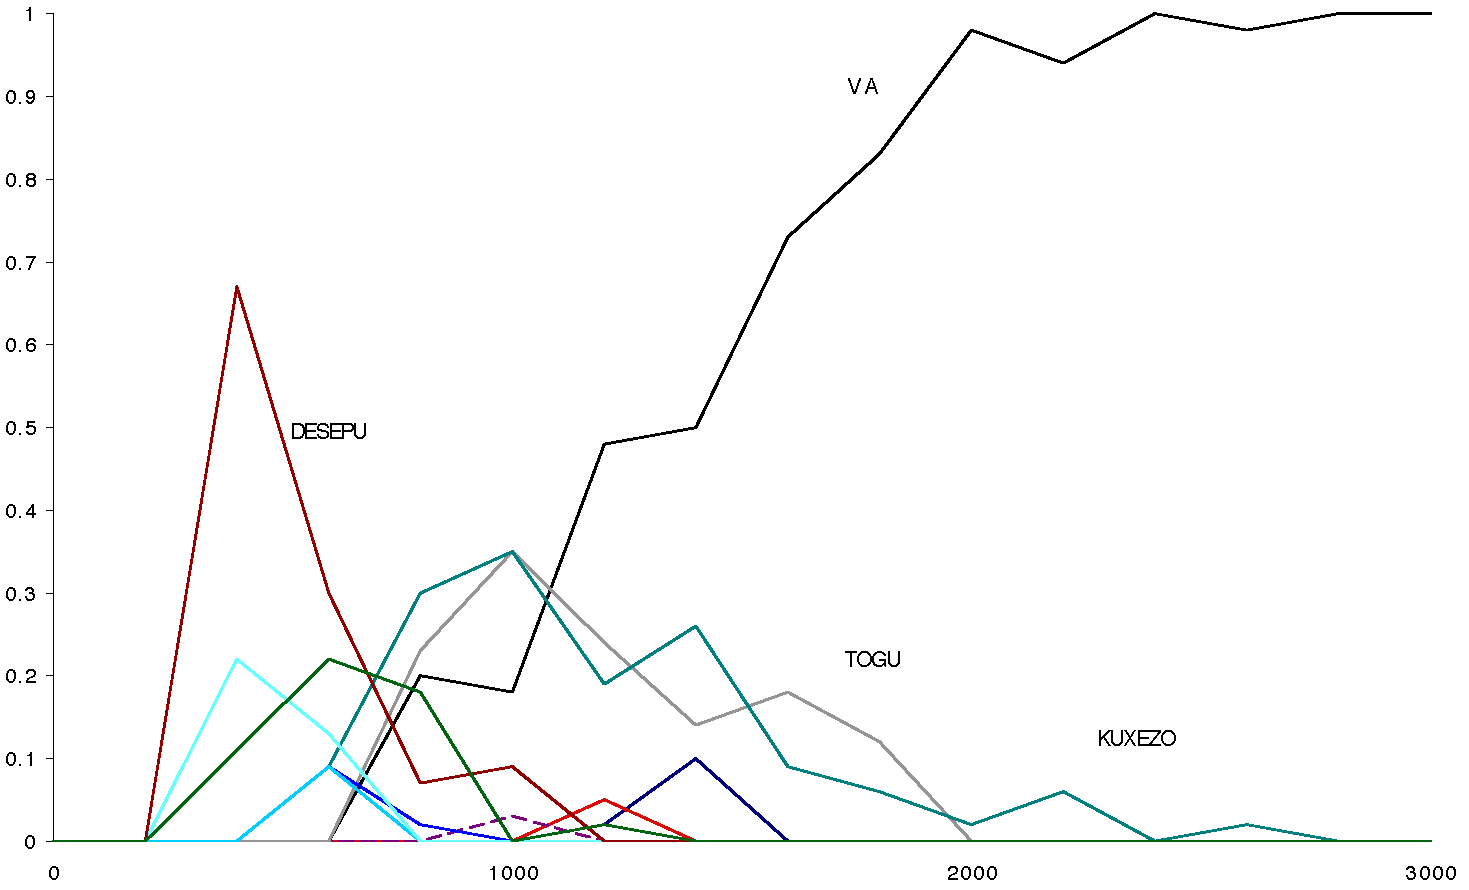
\includegraphics[width=.80\textwidth]{chap7/figs/rf.pdf}}
\caption{\label{RF-diagram}This RF-diagram shows
the frequency of all forms used for the same referent in 
3000 language games, played by a group of 20 embodied
situated agents.}
\end{figure}

The RF-diagram\is{RF-diagram} in \figref{RF-diagram} shows the 
frequency with which certain words were used to communicate 
a particular situation. We see that in
the beginning the word `desepu' has been dominant, then 
there is a period of turbulence in which different 
words compete, but after a while a new word `va' wins 
the competition and becomes the dominant way to communicate 
about this situation. \figref{FM-diagram} shows another\is{FM-diagram}
competition diagram plotting the evolution of the FM-relation, for 
the word form `va', in other words the frequencies of 
all the meanings that co-occurred with the word `va'. 
We see an early peak when `va' was used in 70 \% of the 
games with the meaning [\textsc{b} 0.3125–0.375], i.e. a particular
shade of blue. Then there is a struggle during which additional
distinctions (on the \textsc{red} and \textsc{vpos}-channels) are competing
for the dominant meaning of `va'. 
[\textsc{r} 0.0–0.125] finally becomes dominant. 

\begin{figure}[htbp]
  \centerline{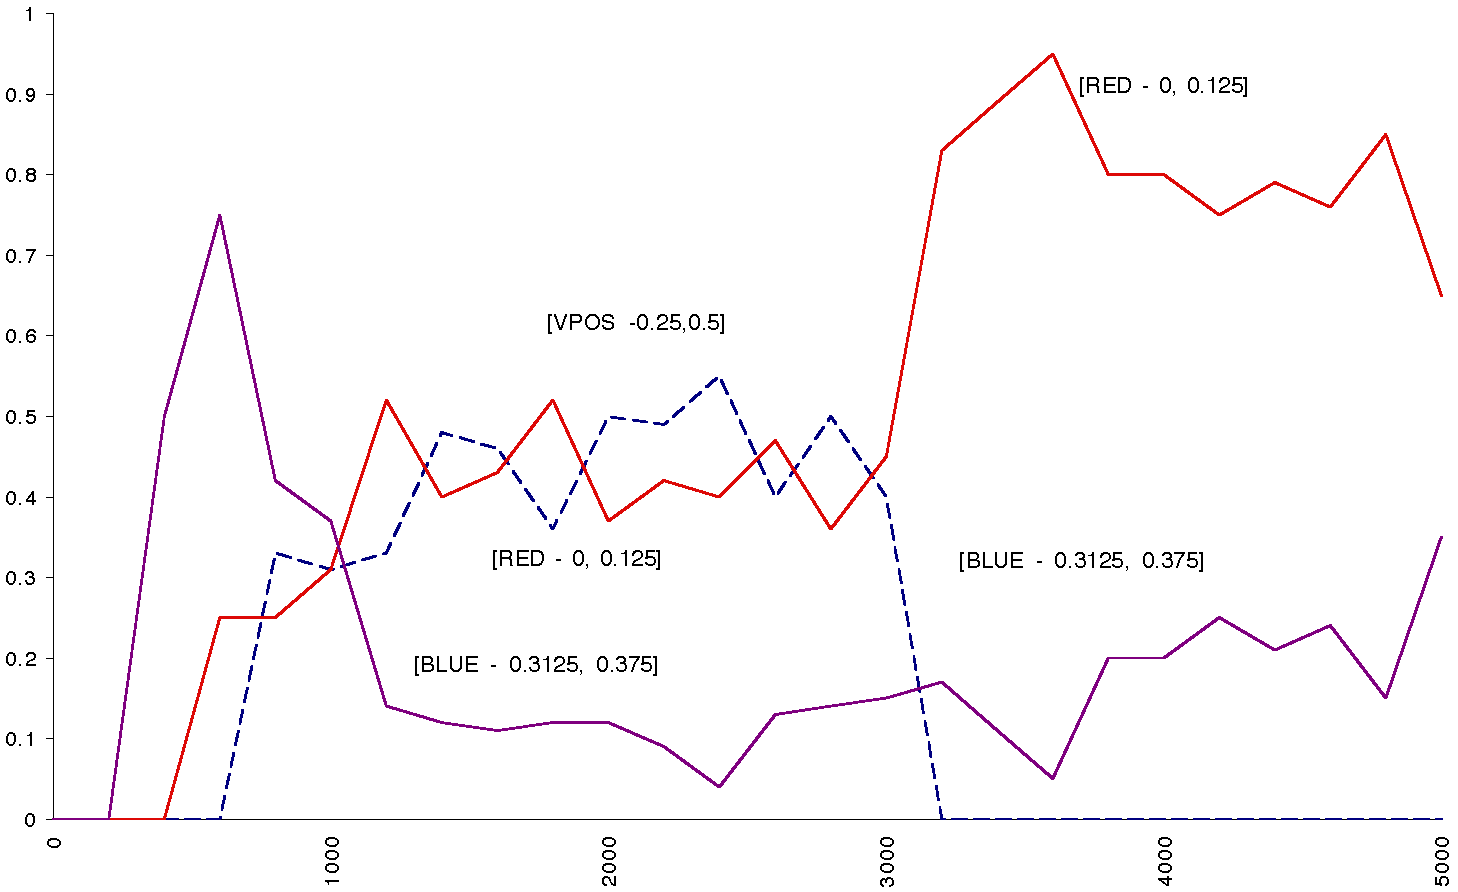
\includegraphics[width=.80\textwidth]{chap7/figs/fm.pdf}}
\caption{\label{FM-diagram}This FM-diagram shows
the frequencies of each form-meaning pair with 
the form equal to `va' in a series of 5000 games.
A disambiguating situation occurs in game 3000
causing the loss of one meaning of `va'.}
\end{figure}

These competition diagrams are an important tool to try 
and make sense of the ontological and lexical evolution
taking place in evolving groups of agents as they are
playing their language games. Typically we pick
a dominating word, for example the word `va' in 
\figref{RF-diagram}, and try to understand
why it has become dominant. 
The FM-diagram for `va' (\figref{FM-diagram}) explains
part of the story. Three stable meanings for `va' have emerged
at \todo{inserted `at' here} around 1000 games: 
[\textsc{r} 0.0–0.125], [\textsc{b} 0.3125–0.375], and [\textsc{vpos} 0.25–0.5]. 
They are all equally adequate for distinguishing the object
`va' designates, and there are no situations yet
that would have forced the disambiguation of `va'. 
In game 3000, the environment (which is continuously 
changing in this experiment) produces a scene in which
a category which was distinctive for the object designated by 
`va' is no longer distinctive. The lexicon adapts 
immediately. Around game 3000 the \textsc{vpos}-based meaning disappeares, 
and the distinction based on \textsc{red} shoots up and becomes dominant. 

\subsection{RMF coherence}

The average frequency of the dominating relations along\is{RMF-coherence}
a particular semiotic dimension is an indication how coherent the
community's language system is along that dimension.
For example, suppose we want to know the coherence along
the meaning-form dimension, in other words
whether there are many synonyms in the lexicon or not.
For a given series of games, we calculate for each meaning
that was indeed used in the series,
the frequency of the most common form
for that meaning. Then we take the average of these frequencies
and this represents the MF-coherence. If all meanings had
only one form, the MF-coherence is equal to 1.0. If two forms
where used for the same meaning with equal frequency, 
MF-coherence is 0.5. When plotting the
MF-coherence we can therefore follow the tendency towards
an increase or decrease of synonyms.

Examining the coherence along the other dimensions is 
equally instructive. Studying the coherence along the FM 
dimension informs us about the degree of ambiguity in the lexicon, 
because it is based on the average frequency of
the preferred meaning for each word. 
When all word forms have only one meaning, the FM-coherence is 
1.0. The more the forms in a language have different 
meanings with non-zero frequencies, the lower the FM-coherence
becomes. 

The coherence along the RM dimension informs us 
about how many possible conceptualisations of the same
situation are used by the population. If RM-coherence is 
high, this means that the population has 
uniform conceptualisations. For every referent, 
all agents typically use the same meaning. 
Usually there are initially many possible ways to conceptualise 
a scene, but there is a tendency 
for agents to view the world in a similar way under
the influence of language because the scores of the 
discrimination trees are affected by success of a 
distinction in language games. I will discuss this 
in more detail in the final section of this chapter.

The inverse relation (MR, between meanings and referents)
tracks the frequency with 
which certain situations are covered by specific
meanings. It informs us about 
the generality of the categories available to the 
agents, assuming that all agents statistically encounter
the same sort of environments. If a particular meaning can
pick out many possible referents in many contexts, this
meaning must be abstract and the agents must have managed
to develop a lexicon that is not tied up completely 
to specific situations. 

\section{The ideal language}

Complex adaptive systems show a tendency to\is{ideal language}
optimise their internal functioning despite the absence of
a global overall control center. For example, 
each species in a single ecology tends to become 
better in exploiting its niche and the global system 
moves towards a balanced equilibrium where different
species play different roles in a complex ecological 
web.\footnote{See examples in \cite{Margulis:1991}.} This book explores the idea that language 
is a complex adaptive system like a natural ecology, 
which is shaped and 
reshaped by the local interactions of autonomous 
agents without a central controlling agency regulating
what linguistic conventions should be adopted. 
We have seen that in computer simulations and experiments
with robotic agents a shared communication system 
emerges, but in how far is this system optimal?\footnote{
See for the discussion on whether languages ever
can be said to optimise: \cite{Kirby:1999}.} 

\subsection{Total coherence}

A first desirable property of a language system 
is perhaps that it is totally coherent along all 
semiotic dimensions. 
In terms of semiotic landscapes, 
this means that the graph consists of unconnected triangles. 
Each object in a specific context has a unique
meaning, each meaning has a 
unique form and picks out a unique referent, and each form 
has a unique meaning and hence a unique referent as well. 
The coherence along all possible dimensions is then always
1.0. Given such a system, the agents would not need to
consider different hypotheses while speaking or listening, 
there would never be any confusion, and a new agent 
learning the language would never be confronted with 
different uses of the same word. 

Such an ideal language has been a dream of many 
philosophers, including Descartes and Leibniz, but 
the investigations reported here show clearly that 
it is not attainable.\footnote{The history of this search for such an ideal language
is discussed by \cite{Eco:1997}.}
A language must be open to the 
expression of new meanings because the communicative 
objectives and the environments which are the subject
of communication keep changing. Hence 
synonymy (incoherence along the MF dimension) is unavoidable
because words are created by some agents not knowing that 
words already exist in the population for the same meaning. 
In addition, one agent 
may ``wrongly'' infer that a certain word has a 
particular meaning due to perceptual anomalies, even though
the same word had already another meaning in the
lexicon. Word-meaning pairs that thus
arise may start to propagate 
in the population and actually supersede the ``original'' 
word-meaning pairs. 

Ambiguity\is{ambiguity} (incoherence along the FM dimension) 
is unavoidable as well for similar reasons. 
The same situation can often be conceptualised in more than 
one way and so an agent guessing the meaning of an unknown 
word or trying to make sense of a word in a particular 
context may easily derive another meaning than the one 
used by the speaker. Perceptual anomalies further aggrevate
the risk that a certain form becomes associated with 
another meaning by the hearer, as we have seen in some
grounded example games earlier on. 

Different conceptualisations of the world (incoherence 
along the RM and MR dimensions) are even harder to 
avoid because every agent develops its own 
ontologies independently and without any direct 
feedback from the other agents. 
The ideal language system is not only impossible to 
attain for autonomous agents engaged in grounded
language games, it would be very 
inefficient to store and use as well because 
new words and meanings would be required for every new 
situation ever encountered. The larger the lexicon,
the harder the task of a language learner to acquire it. 
So there is a trade off between coherence and expressability. 
This is why natural languages constantly try to recruit existing 
words to keep down the repertoire of \enlargethispage{2\baselineskip} 
forms that have to be stored and hence learned.

\subsection{Communicative success despite incoherence}

A grounded language system cannot be fully coherent. 
This implies that communication among autonomous 
embodied agents can only work if their internal 
architectures are capable to handle incoherence. 
Of course, incoherence may not necessarily 
impinge on communicative success. 
Alternative conceptualisations may 
be compatible with the same situations. Agents may not
even realise that their language systems are different
because even though their words have different 
meanings these meanings may always pick out the 
same topic. Thus 
the RMF-landscape in \figref{RMF1} leads to total
success for communicating situation2. Even if 
a speaker uses `tisame' to mean [\textsc{gray}-0.0,0.25] and the hearer
understands `tisame' to mean [\textsc{hpos}-0.5,0.75], they 
still have communicative success. The goal 
of the language game is to find the referent. It does
not matter whether the meanings are the same. The agents
cannot even know which meaning the other one uses
because they have no access to each other's internal states. 

The architecture of the agents in the Talking Heads
experiment has been carefully designed so that incoherence
can be handled. The context
is at every level strongly taken into account. When 
producing an utterance, the meaning of a word is partly
determined by whether
that meaning makes sense in the specific context
of the language game. This makes it possible to 
handle ambiguity. To handle synonymy, agents store several words in 
their lexicons so that they can understand more words
than the ones they prefer themselves. Agents maintain 
different ways to conceptualise reality so that 
they can apply conceptualisations used by others
even though they would not prefer these themselves. 

The agents behave in their own selfish interest to 
maximise success in the game. They increase the score 
of the word-meaning pairs that yielded success and decrease
those that resulted in failure so that next time around 
they are more likely to use that word-meaning pair. 
But a side effect of this behavior is 
that synonymy and ambiguity get damped. Success depends 
on use in the rest of the population. The more 
agents use a word, the more it will have success, 
the higher the scores will be, and the more it will be used. 
The global effect is that the language becomes more
coherent without a central coordinator. 

\section{Damping synonymy and ambiguity}

To conclude this chapter, I now discuss in more 
detail an example of this kind of semiotic dynamics as
gleaned from  an actual experiment with twenty Talking
Heads, taking turns to materialise themselves in two robotic 
bodies at a single physical site. The agents have 
only R, G, B, and gray-scale channels. This 
case study illustrates how the tools introduced in 
the previous section help us to make sense of
the very complex lexical evolution spontaneously 
arising in the system. We have set up the experiment
in such a way that the agents first see a limited set 
of objects. Then we
have progressively added new situations
to the environment (by pasting new figures on 
the white board or reconfiguring existing figures) and studied
the impact on the lexicons and ontologies of the agents.\footnote{
These experiments work were done in strong collaboration with 
Frederic Kaplan, see for example \cite{Steels:1999}.}

\figref{globalsuccess} plots the global 
result of the experiment for 35,000 games. It shows the progressive 
increase in environmental complexity (after every 
5000 games) and the average communicative and discriminative
success in the game. During the final 15,000 games, no new
objects were introduced. 

\begin{figure}[htbp]
  \centerline{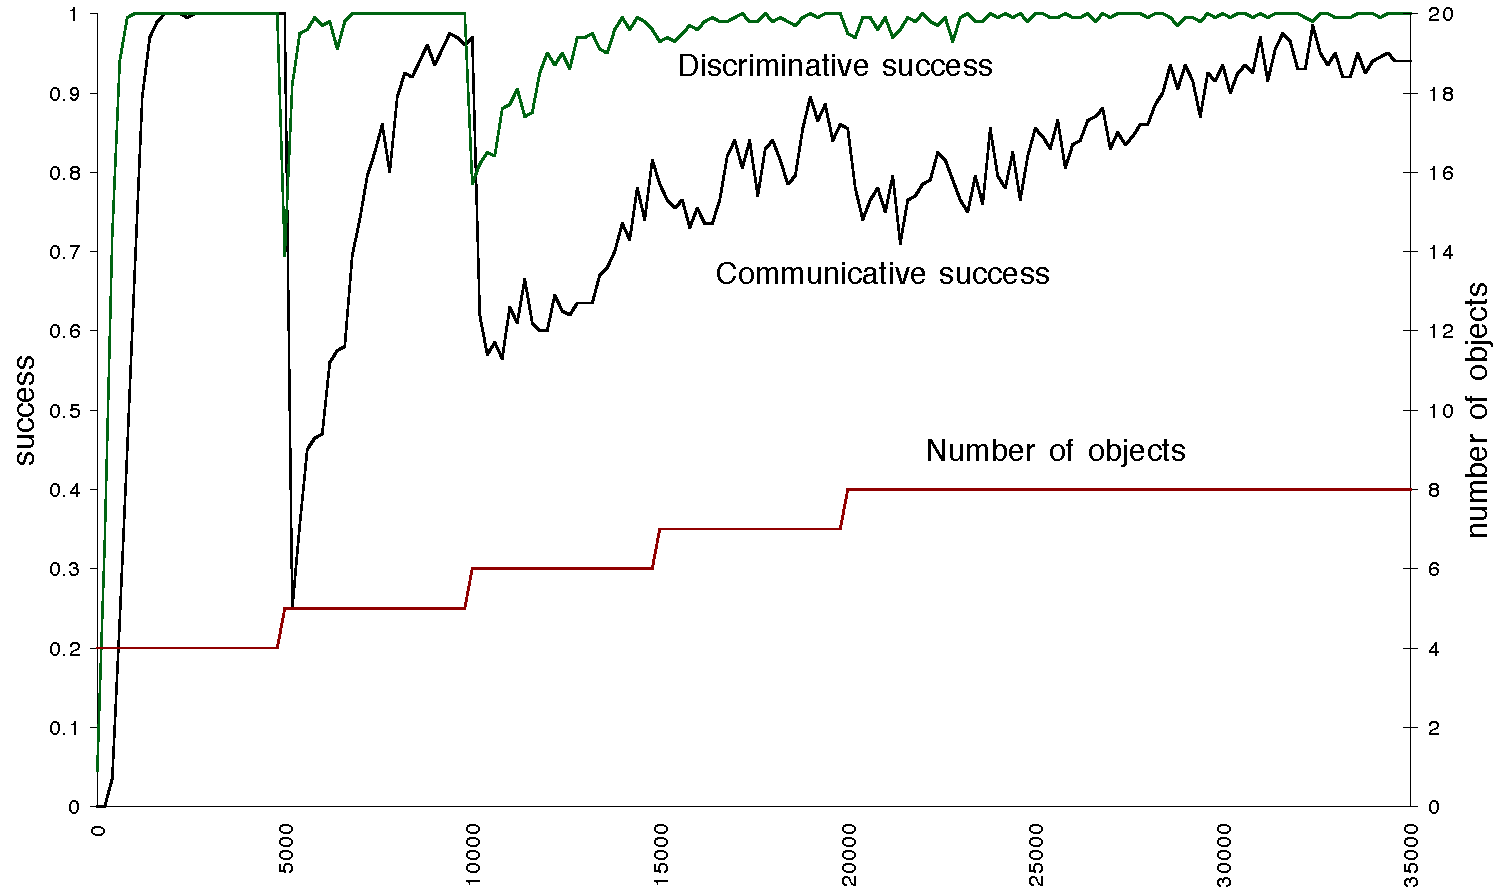
\includegraphics[width=.80\textwidth]{chap7/figs/globalsuccess.pdf}}
\caption{\label{globalsuccess}The graph shows the communicative
and discriminatory success for a series of 35000 language games
played by a group of 20 Talking Heads. The environment 
has progressively been made more complex.}
\end{figure}

We see clearly that the agents manage to bootstrap 
a successful lexicon from scratch in the first 1000 
games. Success then drops every time
the environment increases in complexity but regains as the 
agents invent new words or create new meanings. Progressively 
it is less and less difficult to handle increased
environmental complexity because distinctions are 
already available to cope with the novel
situations, words are less ambiguous, 
and the lexicon is covering more and more meanings. 

\subsection{The story of `fepi'}

\begin{figure}[htbp]
  \centerline{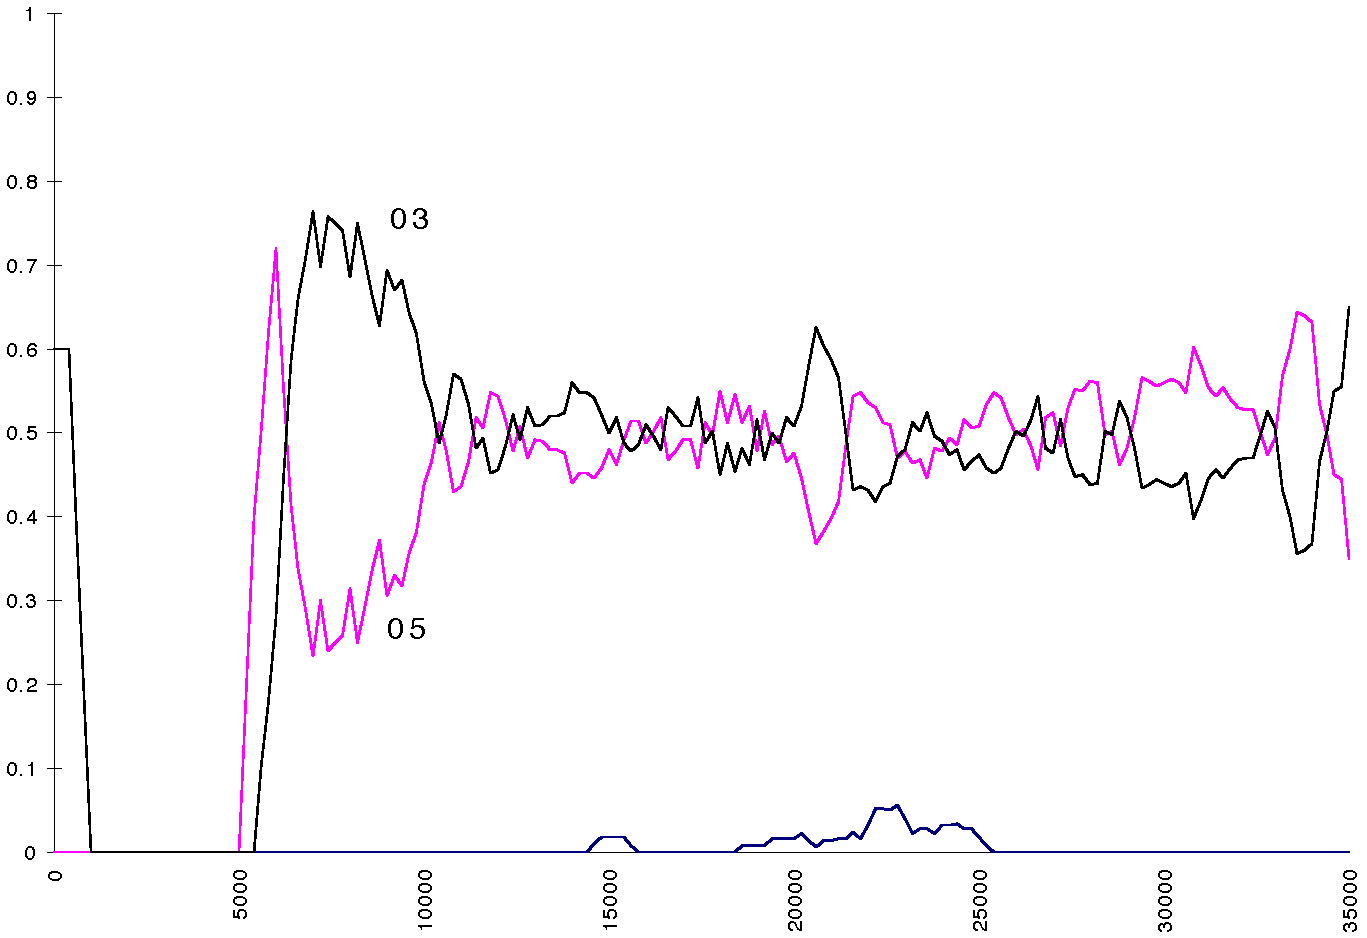
\includegraphics[width=.80\textwidth]{chap7/figs/FR-FEPI.pdf}}
\caption{\label{fr-fepi}FR-diagram showing the frequencies
of the objects referred to by the word
`fepi'. `fepi' is consistently used for \emph{O3} as well as
\emph{O5}.}
\end{figure}
Only looking at macroscopic measures like communicative
success hides away the
interesting rich lexical dynamics that unfolds
in the population. Let me examine just one word, `fepi'. 
By looking at the FR-diagram, we see that this word is 
used consistently for identifying two objects
(\emph{O3} and \emph{O5}) in a certain set of contexts
(\figref{fr-fepi}). 

\begin{figure}[htbp]
  \centerline{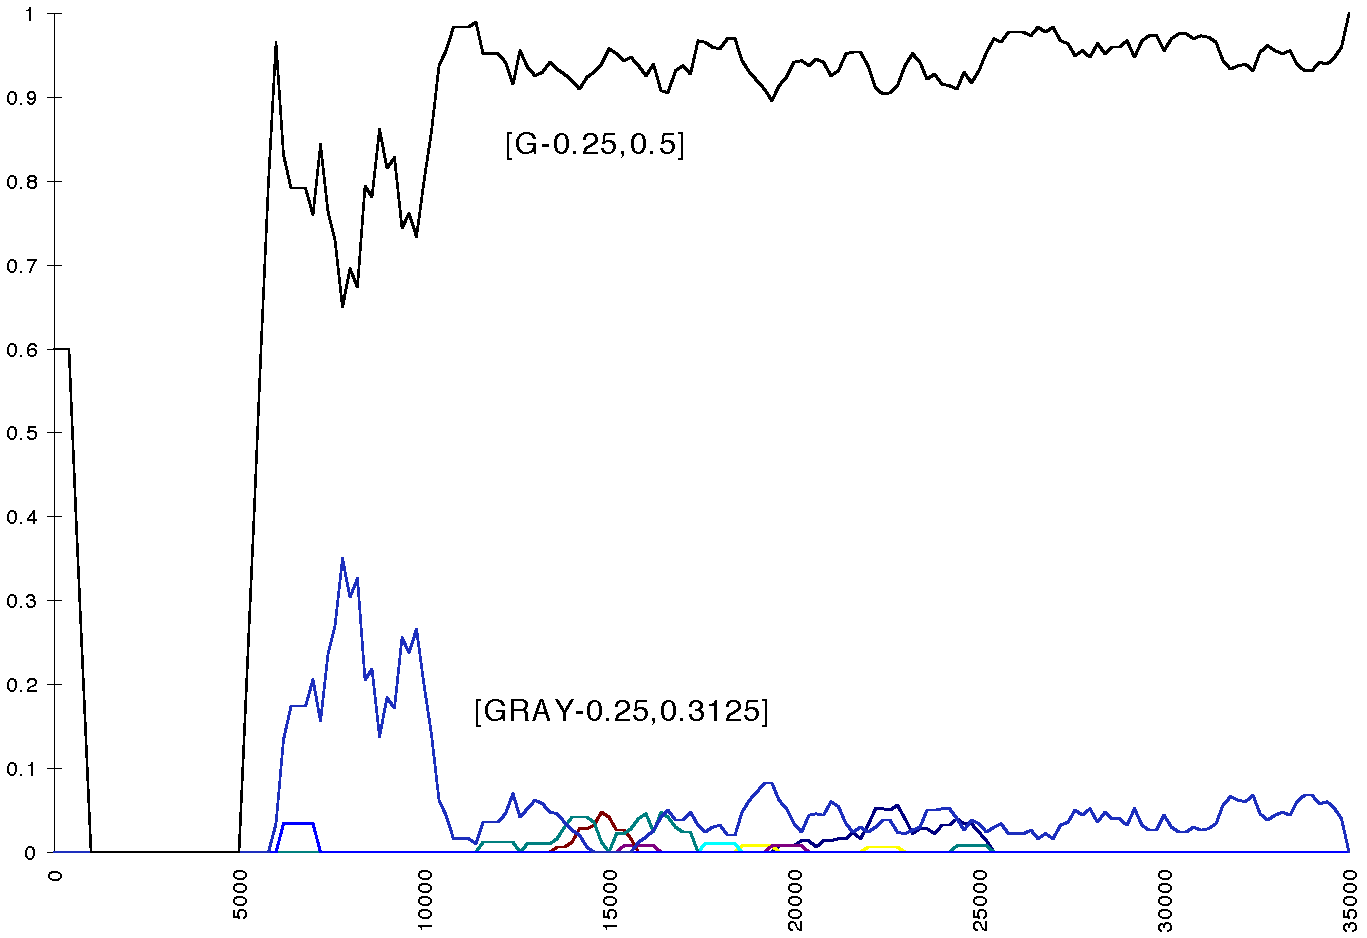
\includegraphics[width=.80\textwidth]{chap7/figs/FM-FEPI.pdf}}
\caption{\label{fm-fepi}FM-diagram showing the different
meanings of `fepi'. One meaning [\textsc{g} 0.25–0.5] dominates.}
\end{figure}
We can see the meanings of `fepi', by 
inspecting its FM-diagram (\figref{fm-fepi}). 
The dominant meaning of `fepi' is 
a particular shade of green [\textsc{g} 0.25–0.5]. There are 
some other competing meanings (including [\textsc{gray} 0.25–0.3125])
but most of them are hardly ever used. We observe clearly 
the tendency for ambiguity to get damped. 

What about synonymy? Let us look at the 
MF-diagram of [\textsc{g} 0.25–0.5], so that we can
see whether there are any other words in use for expressing
the same meaning (\figref{g02505.f}).
`fepi' has indeed emerged as dominant for this meaning, but 
this has not been without an intense struggle.
The tendency for synonymy to get damped is clearly present. 
Even though the lexicon occasionally destabilises, 
the lateral inhibition and the positive feedback loop between use 
and success causes self-organised MF-coherence. 
There is however something curious going on. 
In the early phases `xu' was dominant. Why did it 
destabilise and how has `fepi' has managed to become the
dominant expression for [\textsc{g} 0.25–0.5]? 

\begin{figure}[htbp]
  \centerline{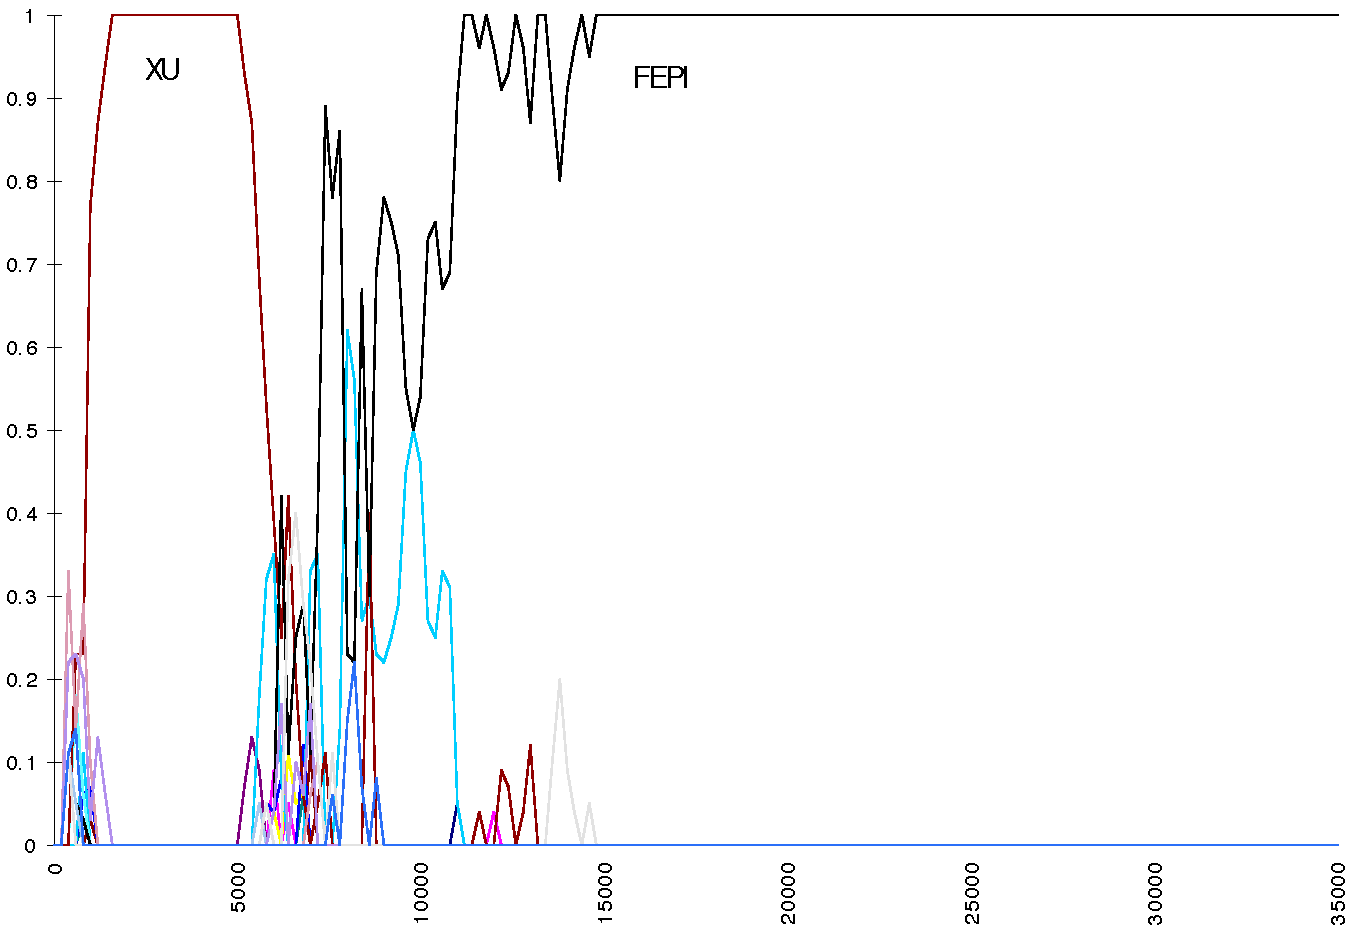
\includegraphics[width=.80\textwidth]{chap7/figs/MF-G-025-050.pdf}}
\caption{\label{g02505.f}MF-diagram showing the
different words circulating in the population for expressing
the category [\textsc{g} 0.25–0.5]. First `xu' dominates and 
then `fepi' wins the competition after an intense struggle.}
\end{figure}

\subsection{The story of `xu'}

When inspecting in more detail the game traces,
we see that `fepi' is created in game 328 by agent-3, playing the
role of speaker, in order to refer to object \emph{O3} using 
the meaning [\textsc{g} 0.25–0.5]. Agent-19, the hearer in the same 
game, acquires the same meaning for [\textsc{g} 0.25–0.5]. In one sense,
we could say that agent-19 has learned this meaning of `fepi' from
agent-3 but that is not entirely accurate. Agent-19 
has constructed a possible meaning for `fepi' and this happened
to be the same as the one used by agent-3,
but this is partly accidental. 
Agents only indirectly learn the language from others. They construct
a language which is compatible with the language used by others. 
Coherence among the individual
language systems occurs through the positive feedback between
language use and communicative success.

`fepi' entered into the lexicon to refer to \emph{O3}, but we see
from the RF diagram for \emph{O3} (\figref{RF-O3a}) that 
`xu' was already well established for \emph{O3} and initially 
`fepi' had no success at all. 
So the puzzle is still there, how did `fepi' manage to 
overtake `xu'? 

\begin{figure}[htbp]
  \centerline{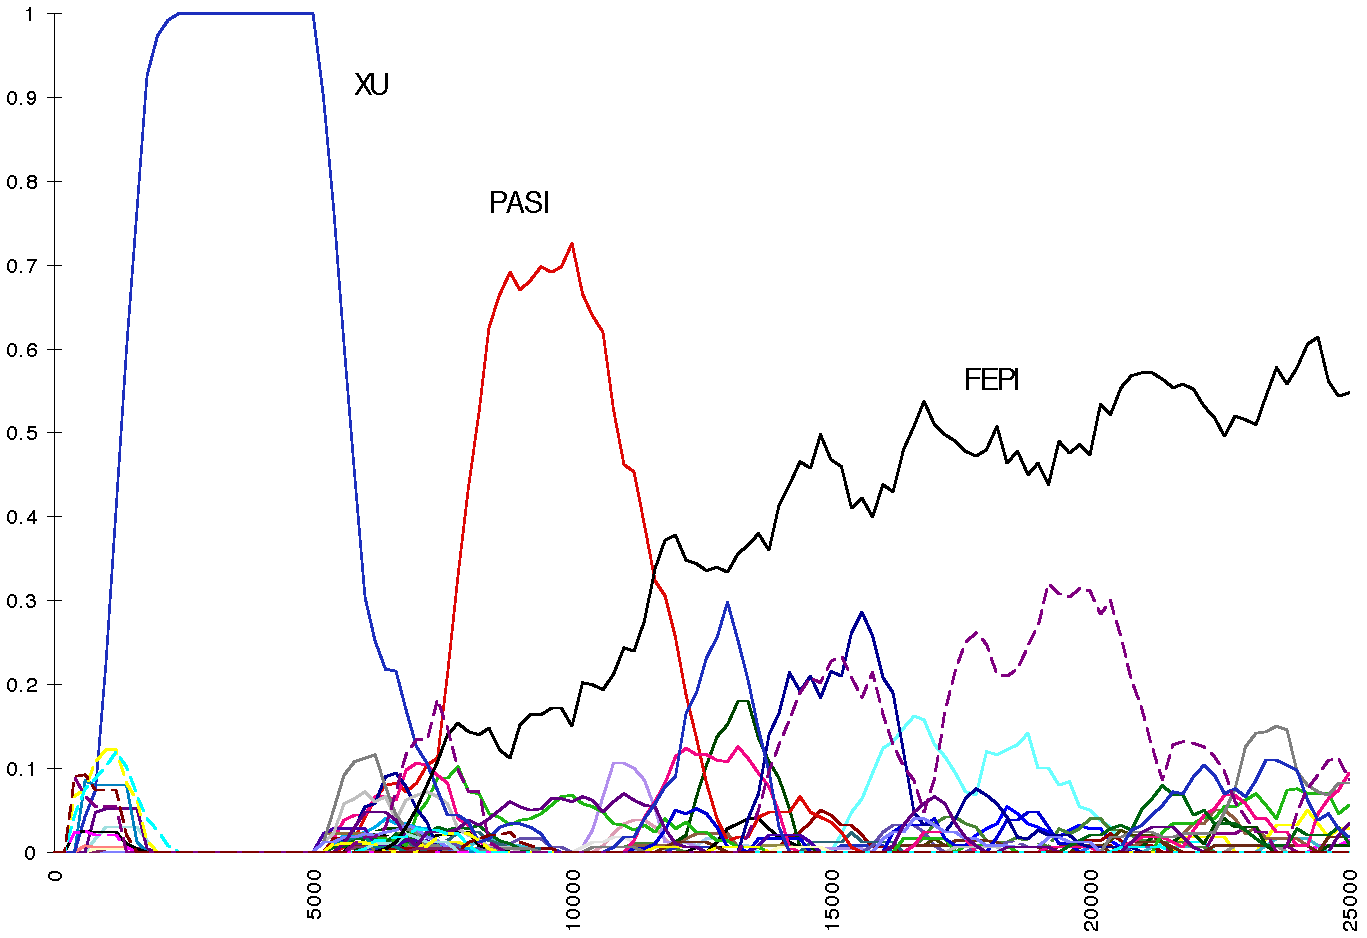
\includegraphics[width=.80\textwidth]{chap7/figs/RF-O3.pdf}}
\caption{\label{RF-O3a}RF-diagram showing the different
words being used for identifying \emph{O3}. Initially `xu' 
dominates }
\end{figure}
Let us look at the different meanings of `xu' on 
a magnified scale by 
inspecting the FM-diagram of `xu' (\figref{FM-XU.f}). 
Only the first 10,000 games are shown because after
that `xu' is no longer used. In the first 5000 games,  
`xu' has the same dominant meaning as `fepi', namely
[\textsc{g} 0.25–0.5]. There are some other meanings 
associated with `xu', which are all effective 
to conceptualise \emph{O3}.

\begin{figure}[htbp]
  \centerline{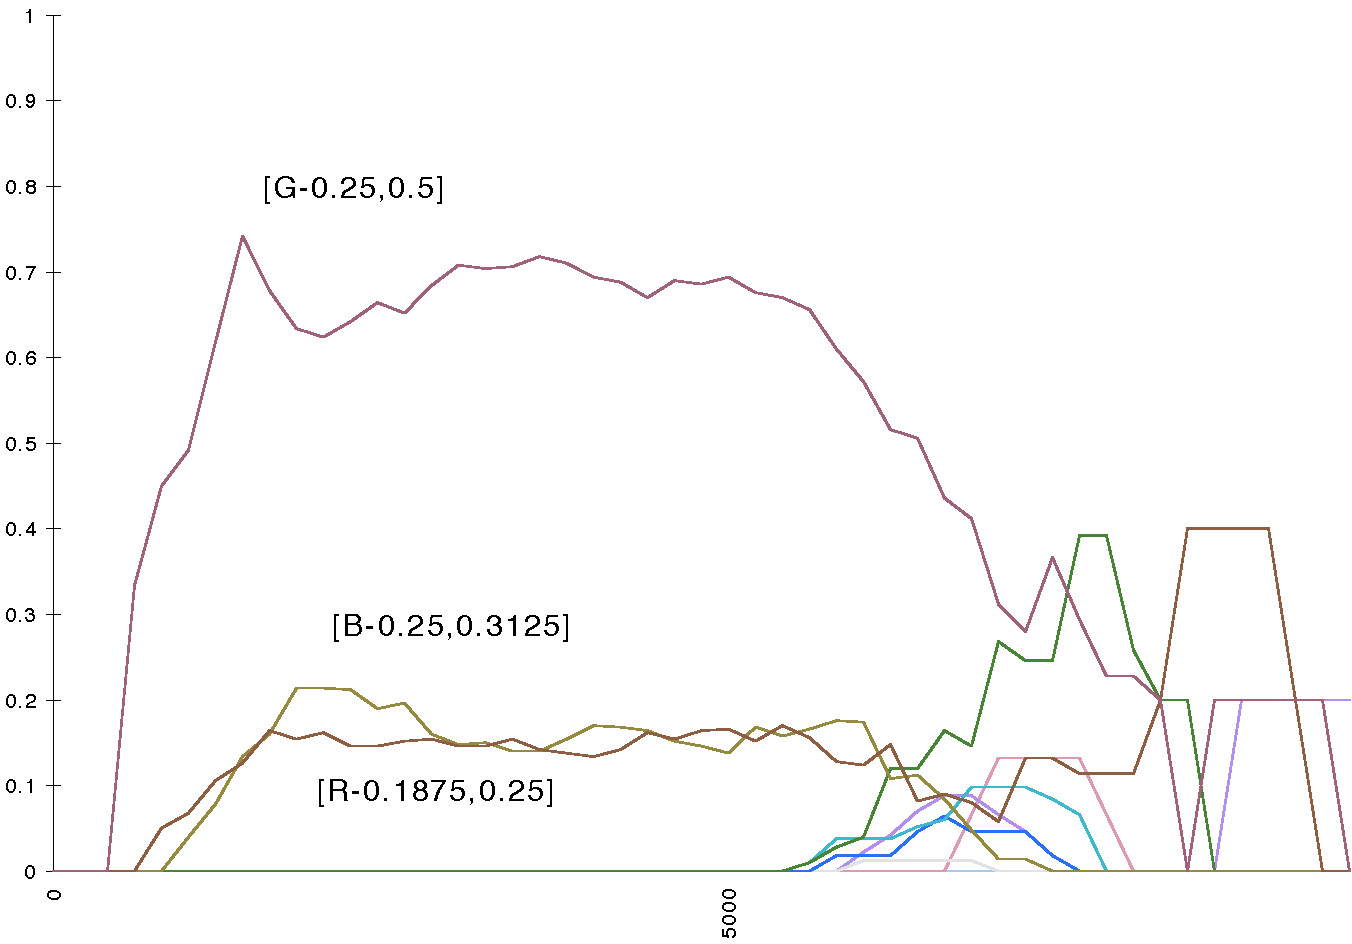
\includegraphics[width=.80\textwidth]{chap7/figs/FM-XU.pdf}}
\caption{\label{FM-XU.f}FM-diagram showing the different
meanings of `xu'. After game 5000, the meaning of `xu' becomes
unclear and the word falls in disrespute.}
\end{figure}

\subsection{The entry of \emph{O3}}

The mystery is unveiled by looking at what
happened when \emph{O3}, a new object, entered the environment 
around game 5000. The word `xu' now not only picks out
\emph{O3} in certain contexts but \emph{O5} as well. Hence 
games where both objects are occurring fail and consequently 
the association between `xu' and [\textsc{g} 0.25–0.5] is 
weakening. Closer examination reveals that \emph{O5}'s green value
is a bit lower (in the range [0.25,0375]) than that of \emph{O3}
(which is in the range [0.375,0.5]), so that a more refined
distinction on the G-channel is necessary if both objects
occur in the same context. 


\begin{figure}[htbp]
  \centerline{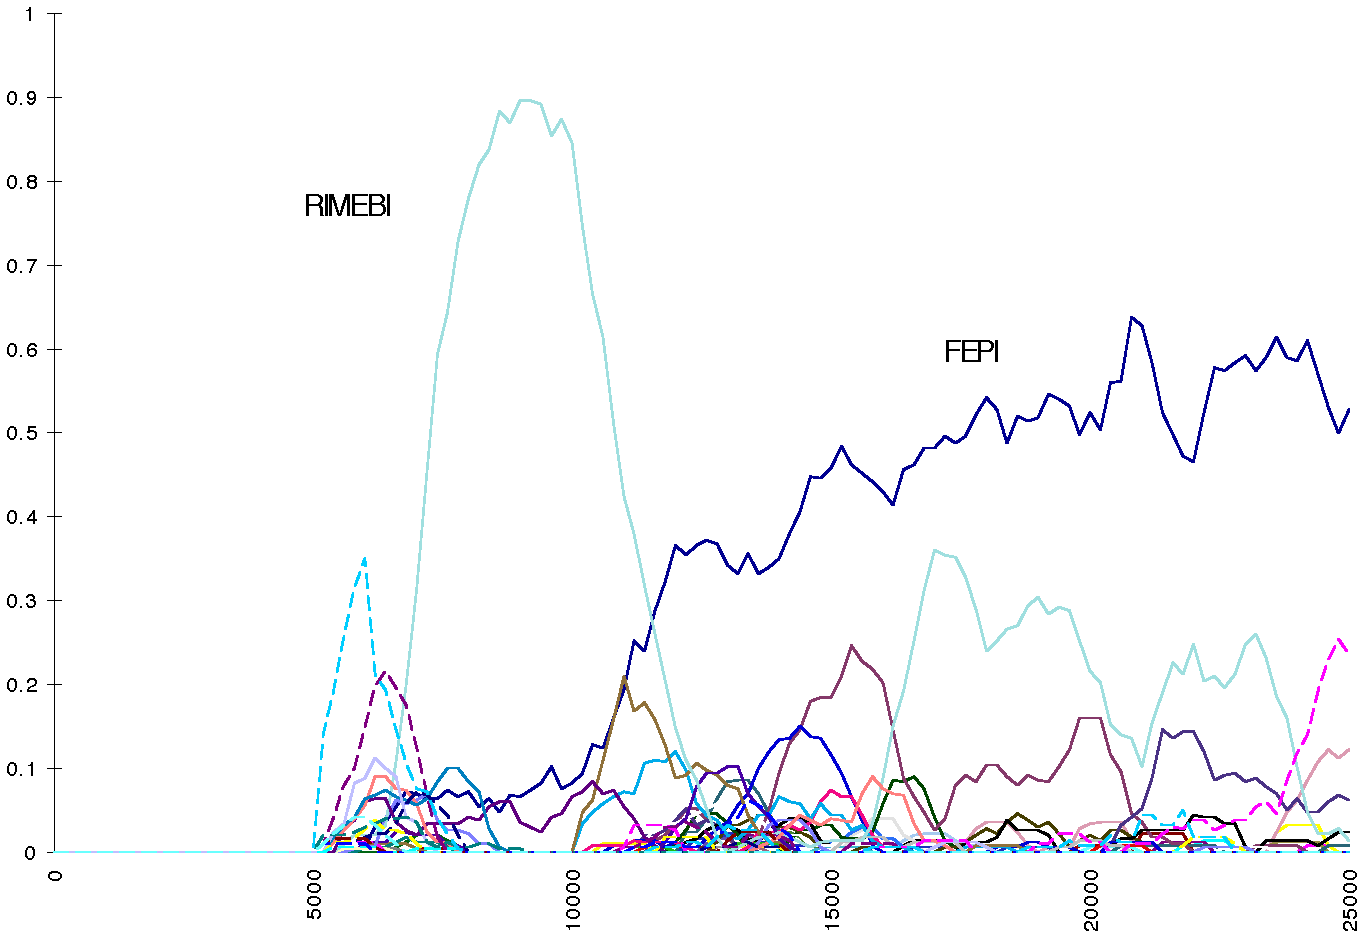
\includegraphics[width=.80\textwidth]{chap7/figs/RF-O5.pdf}}
\caption{\label{RF-O5}RF-diagram showing
the different words used for \emph{O5}. Initially a word 
`rimebi' dominates. It destabilises and `fepi' takes over.}
\end{figure}

As seen from the RF-diagram in \figref{RF-O3a}, `xu' is no
longer used for \emph{O3}. Instead the word `pasi' comes to 
dominate. `pasi' has indeed the more specific 
meaning [\textsc{g} 0.375–0.5] which is only applicable to \emph{O3}, 
not to \emph{O5}. At the same time we see from the RF-diagram 
for \emph{O5} (\figref{RF-O5})
that the word `rimebi' initially dominates for designating \emph{O5}. 
`rimebi' has the more specific meaning [\textsc{g} 0.25–0.375] which 
is not applicable to \emph{O3}. 
The more general word `xu' is still useful in some 
contexts where the
refined distinction is not necessary (for example where 
either \emph{O3} or \emph{O5} is present but not both). So we would expect
that `xu' continues to exist. However this is not the case. `xu'
loses out completely and its role is taken over by `fepi'. 
\clearpage
Understanding why this is the case
tells us a great detail about the kind 
of hidden semiotic dynamics that takes place. `xu' loses its
strength because (1) it fails in games where its meaning
is \todo{inserted `is' here} not distinctive enough so that its score goes
down, and (2) because there 
are other meanings competing with `xu' which do not 
have strong alternatives and are therefore
less prone to failure. This is notably the case for
`fepi'. `fepi' carries the more general meaning of green
and does not have competitors. It therefore overtakes
`xu'. 

This example shows many things. Clearly
lexical dynamics can be very complicated, despite the 
fact that the underlying mechanisms are relatively 
simple. Complexity comes partly from the complexity of
the environment that continues to challenge the agents
with novel , and partly from the internal 
complexity the semiotic dynamics spontaneously generates. 
There are strong tendencies in the agents' lexical systems
towards FM and MF coherence, 
in other words towards shared lexicons. These tendencies
are not due to a central controlling authority which 
has a global view of the lexicon and dictates to the 
agents what they should do but because incoherent 
form-meaning pairs do not resist when the environment 
changes. As we have seen, the word `fepi' could 
overtake `xu', because `xu' had alternative meanings that 
caused failures in novel situations and `fepi' did not. 
`fepi' had a higher coherence and therefore survived, even
though `xu' was used more often but with an 
ambiguous meaning. 

\section{Rousseau's paradox}

The self-organised coherence of lexicons is an important\is{Rousseau's paradox}
outcome of the experiments, but what about the other
semiotic dimension, the relation
between situations and their conceptualisation? 
In how far do the agents use the same 
conceptualisations of reality in the same situations
(RM-coherence) and in how far do they pick out the same topics
given the same meaning (MR coherence). Many different ways
to conceptualise reality may exist side by side and if
each one can be expressed, it would lead to successful
communication. So there is 
less a clear pressure to make the RM-coherence increase. 
The advantage of high RM-coherence is that the agents 
are more uniform in their behavior, so that fewer 
hypotheses need to be considered and the acquisition of 
the lexicon by virgin agents is easier. 

\subsection{Universality versus relativism}

This raises a fundamental question, which has been\is{linguistic relativism}
heavily debated throughout the history of 
philosophy, namely in how far have different languages
different ontologies and in how far does the use of a 
language influence ontological coherence in 
a population. From one point of view, words are seen as labeling 
existing (innate or learned) categories, and so the problem
of learning a lexicon consists in learning 
the association between unknown labels and \enlargethispage{1\baselineskip}
known internal categories.\footnote{
``The speed and precision of vocabulary acquisition 
leaves no real alternative to the conclusion that the 
child somehow has the concepts prior to 
experience with language, and is basically learning 
labels for concepts that are already part of his or 
her conceptual apparatus.'' p.21. in \cite{Chomsky:1987}.}
On the other hand, ethnologists and linguists studying 
non-European languages almost invariably arrive at the 
conclusion that there are profound differences between 
languages, not simply in which words they use but also 
in which way they conceptualise reality. This implies
that there is a kind of co-evolution between language
and meaning.\footnote{The best known representative of 
this position is \cite{Whorf:1956}. 
See for a wider discussion \cite{Lee:1996}.}

Here is a seemingly trivial example of the interaction 
between language and meaning. In French, the second singular person
pronoun (`you') has two forms: 
`tu' and `vous'. Textbooks say that the first is colloquial 
and the second form is polite. A speaker is therefore
required to categorise the social relation between himself
and the hearer, which he is not forced to do in English. 
But polite/colloquial is too simplistic to capture the 
underlying usages. The categorisation of the speech 
situation is quite subtle, possibly incorporating
age differences, professional status, 
class differences, pragmatic context, speaking 
style, etc. Someone learning to speak French must not 
only learn that `you' has two forms but also what the 
subtle distinctions are between the situations where 
you use one or the other. If you think learning this distinction
is difficult, just consider Japanese, where there are 
dozens of words for `I', some of them listed in \tabref{tab:7:japanese}.


\begin{table} 
\caption{Words for `I' in Japanese}
\label{tab:7:japanese}
\begin{tabular}{llll}
\lsptoprule
A            &  Chin       &      As-shi    &        Fu-sho\\
A-i          &  Da-i-ko    &      A-ta-i    &        Ge-kan\\
A-ta-ki      &  Ge-se-tsu  &      A-ko      &        Da-ra\\
A-ta-ku-shi  &  Ge-sho     &      A-re      &        Fu-bin\\
A-te         &  Gi-ra      &      A-shi     &        Fu-ko-ku\\
A-ta-shi     &  Go-jin     &      Bo-ku     &        Gu           \\
\lspbottomrule
\end{tabular}
\end{table}

Here is another example which is more related to 
the perceptually grounded distinctions we 
are studying here. To categorise space, a viewer 
typically imposes a frame of reference 
on the scene before him and categorises regions and positions in
terms of this frame of reference. For example, standing in front of
a chair we could say in English `the table is to the right of the chair', 
where `to the right of' designates an area to the right
within the frame 
of reference relative to axes emanating from the observer. This 
seems the most natural and simplest way to categorise space
and it is used by the Talking Heads when they expand the 
\textsc{hpos} channel. However, there are quite a few languages
which impose an absolute frame of reference, see \cite{Levinson:2006}. 
For example, the Tenejapans from Chiapas, Mexico 
speak a Mayan language known as
Tzeltal. They live in a mountaneous region that is generally 
sloping north-northwest. They use this regional characteristic
to introduce an absolute frame of reference with three distinctions: 
uphill, downhill, and across. Standing in front of the chair, they 
would literally say something like
`standing at its uphill chair the table', in other words, 
`the table is uphill from the chair'. 
The spatial categories left, right, front, back, etc. simply 
do not exist in Tzeltal.
Something that is `to the left' from the viewpoint
of English could be `downhill', `uphill', or `across' depending
on its absolute position. 
If we want to translate `to the left of' 
in Tzeltal, we first have to conceptualise the global reference
frame that is valid in the situation being described,  
and only then we can choose whether `uphill', `downhill', or `across'   
are appropriate translations. It could be argued that 
these differences are purely due to differences in 
lexicalisation. But this is not so. 
An absolute frame of reference
has not only an impact on language but also deep implications
for other cognitive tasks. Psychologists have invented 
non-verbal tasks where speakers of Tzeltal make other spatial
inferences than Europeans. Ignoring such profound 
cultural differences is therefore a sure recipe for
disastrous misunderstandings.

The degree of sharing (or non-sharing) of an 
ontology in a group raises the paradox, first 
expressed by Jean-Jacques Rousseau. Language requires a
sufficiently shared categorisation of reality, otherwise 
no communication is possible. But, if every language 
employs its own 
categorisation (even if there are large overlaps), how is a
particular individual entering a language community supposed to
know the categorisation implicit in his or her
language? It is clear that language 
helps foster shared meaning because meaning is transmitted 
through language, for example when a speaker explains the meaning
of a word to a hearer. On the other hand, successful 
language interaction already requires at least some shared
meaning, how could the system otherwise bootstrap itself?
So we have a chicken and egg situation, a causal 
circularity that somehow must be broken. 

\subsection{Ontological coherence}

The Talking Heads experiment shows a way to resolve\is{ontological coherence}
this paradox. Different agents develop their own 
ontology in a selectionist fashion,
using the growth and pruning dynamics discussed in \chapref{chap:4}. 
Because there is some randomness in the growth
process and because different agents see different cases
in which other channels may be salient, it is highly
unlikely that they all end up with exactly the same 
set of categories, even though 
agents operating in the same environment with a similar 
sensori-motor apparatus will develop similar distinctions. 

On the other hand, the coupling between the conceptual
and lexical layer discussed in the previous chapter
causes a strong interaction between the two. Those 
distinctions whose lexicalisations are the most successful 
are preferred, and the scores
of categorisers is influenced by the outcome of the 
games in which they were used. This structural coupling
causes a progressive coordination of the ontology and 
the lexicon of the agents, even though ontologies will 
never be completely identical. 

\figref{coh} shows the result of some experiments 
focusing on ontological coherence (i.e. RM-coherence). 
The agents reach a close to 100 \% discriminatory 
success, and coherence climbs to 75 \%. 
Multiple solutions are possible, and so there is no reason why the 
agents would have completely convergent ontologies.

\begin{figure}[htbp]
  \centerline{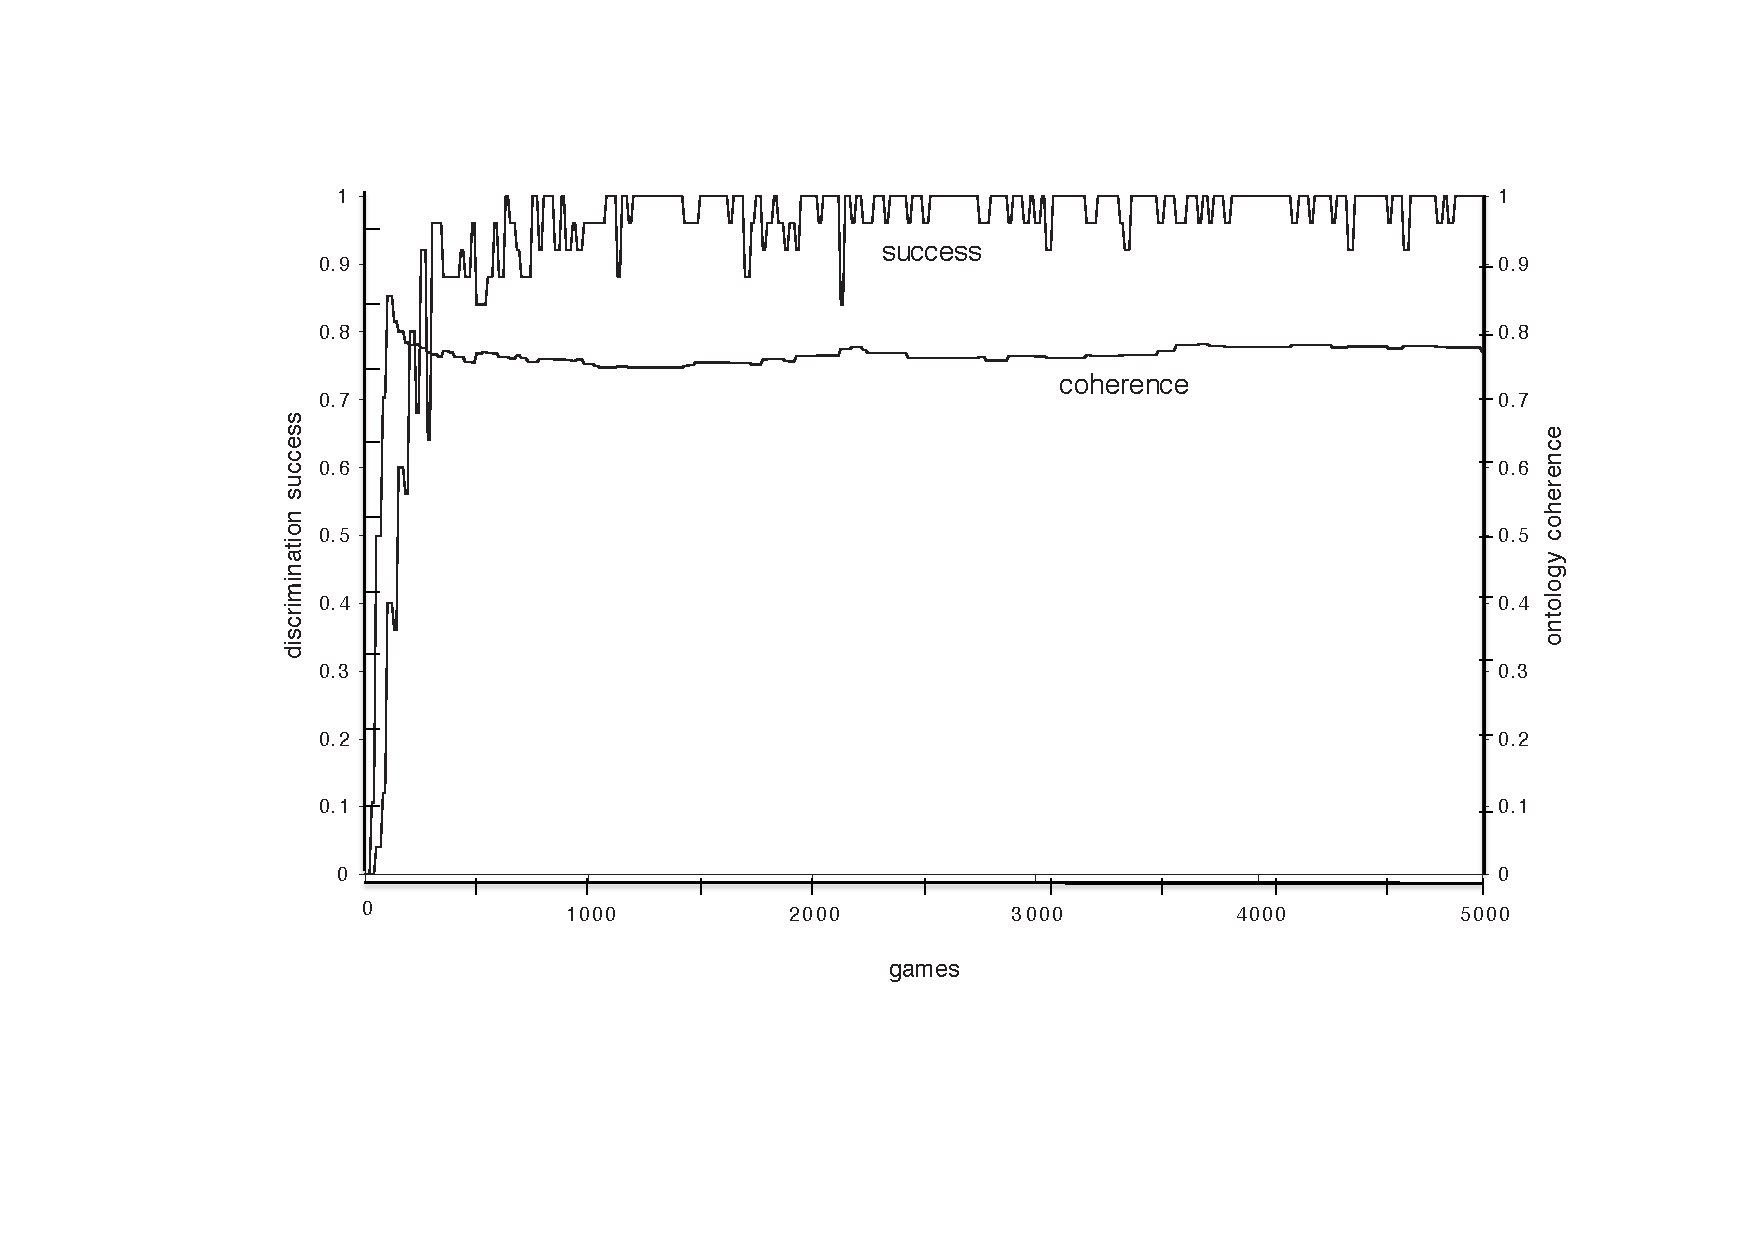
\includegraphics[width=.80\textwidth]{chap7/figs/coh.pdf}}
\caption{\label{coh}This figure shows the discrimination
success as well as the ontological (RM) coherence for
a series of 5000 discrimination games in a group of 10 agents.}
\end{figure}

A more fine-grained way to visualise the emerging
coherence between the agents' ontologies is 
through a {\itshape coherence web} (see \figref{cohweb}). 
There is an axis for each agent as well as
a line emanating from the center of the web.
Let \emph{a1} and \emph{a2} be two 
agents, then \emph{a1}'s line intersects with \emph{a2}'s axis at the 
level of coherence between \emph{a1} and \emph{a2}. For example, if \emph{a1}
and \emph{a2} have a 50 \% ontological coherence, then \emph{a1}'s
line intersects \emph{a2}'s axis at point 0.5. The intersection between 
an agent's line and its own axis represents the average 
coherence of this agent with respect to all the other
agents. When there is little 
coherence, the lines cluster around the center of the cobweb. 
As coherence increases, the lines approach more and more the edges
of the diagram. If all lines end up exactly
on the edges, there is complete coherence. Similar coherence
webs can be constructed for the other semiotic 
relations studied earlier.  

The evolution in the coherence webs in \figref{cohweb} shows clearly that the agents are 
coordinating their ontologies, despite direct feedback 
about the meaning of a game. Feedback only comes from 
the pointing through the external world. More experiments
need to be done to with more channels so that the 
set of possible alternative conceptualisations is 
sufficiently significant to investigate the co-evolution 
of language and meaning more precisely. Nevertheless, 
the experiments show that ontologies can be coordinated
without needing to be innate. 

\section{Conclusions} \enlargethispage{1\baselineskip}

The experiments reported in this chapter have
demonstrated that 
the various mechanisms introduced in earlier chapters
not only work in computer simulations but also in 
experiments with embodied situated agents. 
The grounding of language games in physical 
reality introduces perceptual and behavioral anomalies 
which may cause failures and additional ambiguities
in the lexical systems of the agents. However the 
mechanisms introduced before, particularly the 
forces damping synonymy and ambiguity, still prove to 
be adequate to lead the population towards a 
coherent successful language system. 

The lexical and ontological evolution observed even 
in small populations of agents quickly becomes 
too complicated to investigate by hand. I therefore
introduce a number of tools, such as the semiotic
landscape, the coherence diagrams, and the coherence
web. We clearly need more of these tools and we 
need to study additional properties of emergent 
lexicons, such as the semantic relations between 
the words and how they may evolve. 

\begin{figure}[h]
\centerline{
 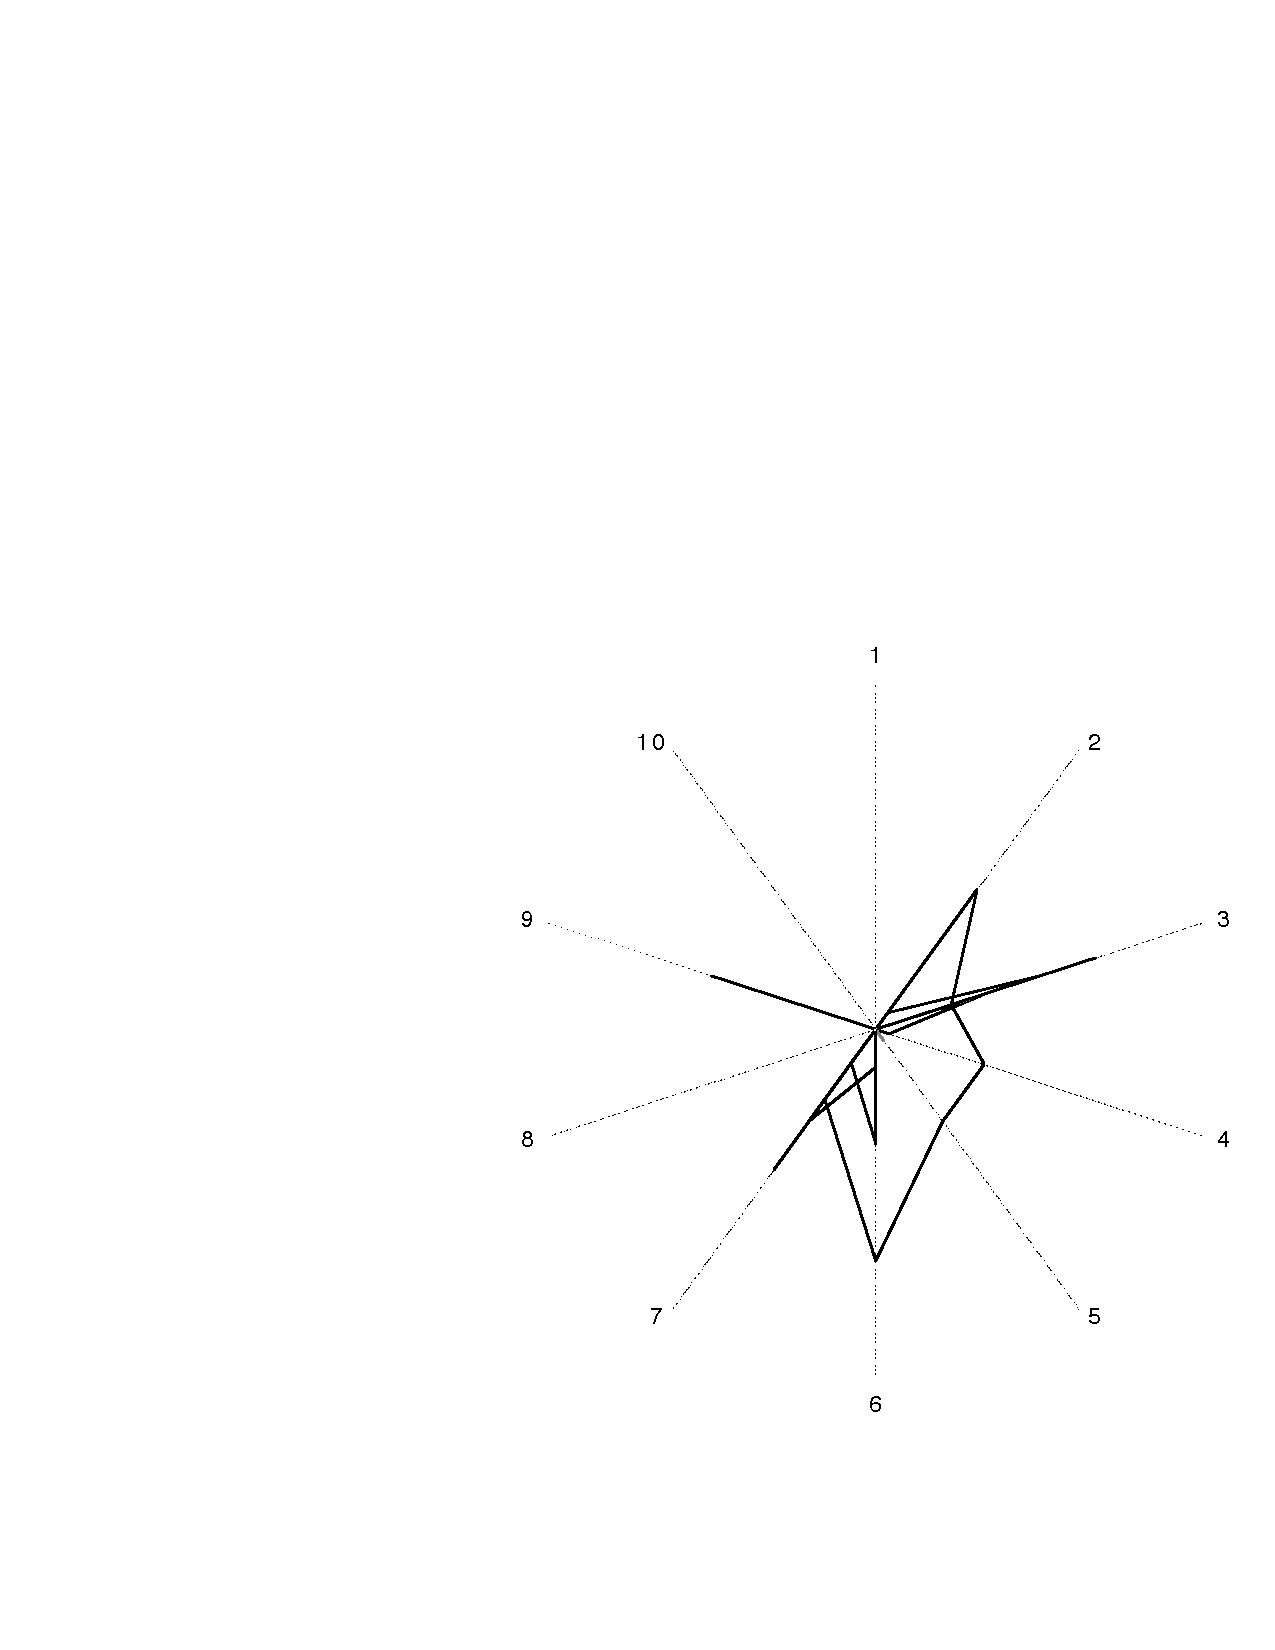
\includegraphics[width=.32\textwidth]{chap7/figs/com-2.pdf}
 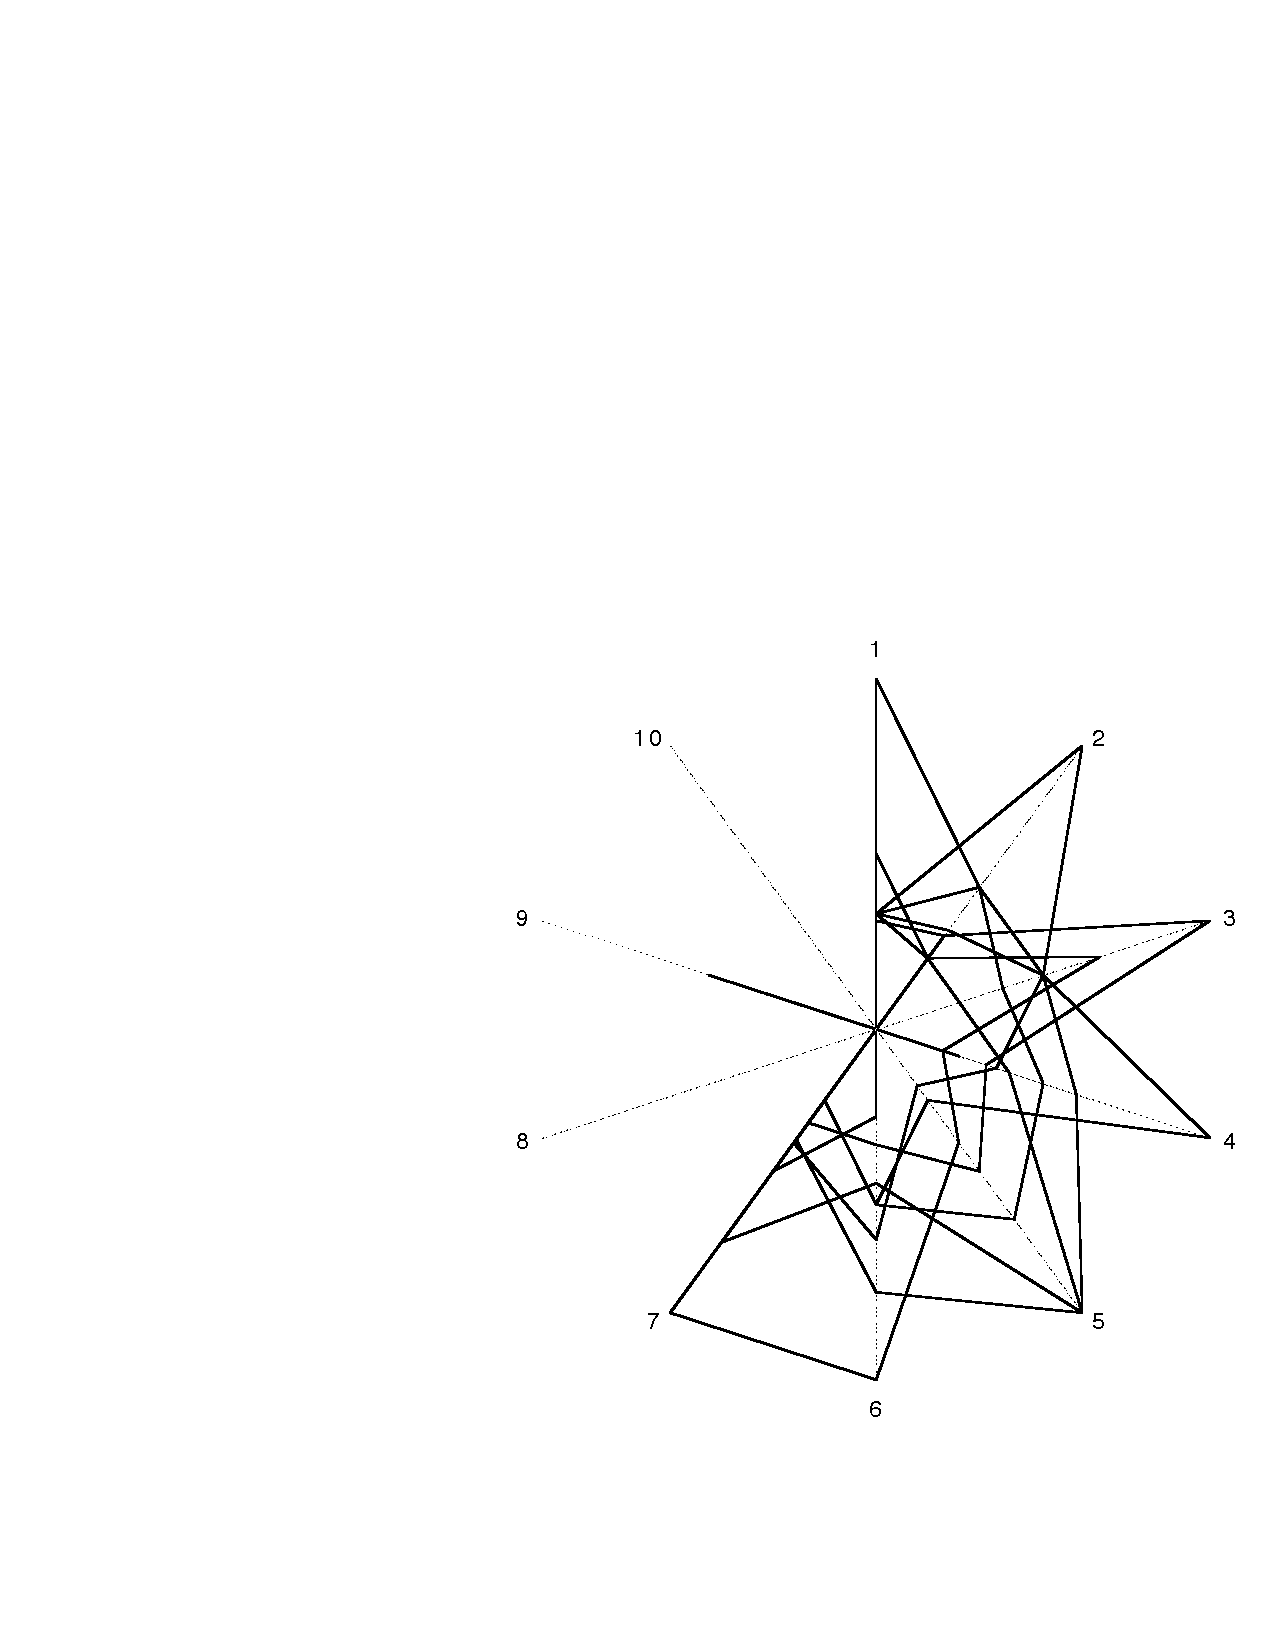
\includegraphics[width=.32\textwidth]{chap7/figs/com-3.pdf}
 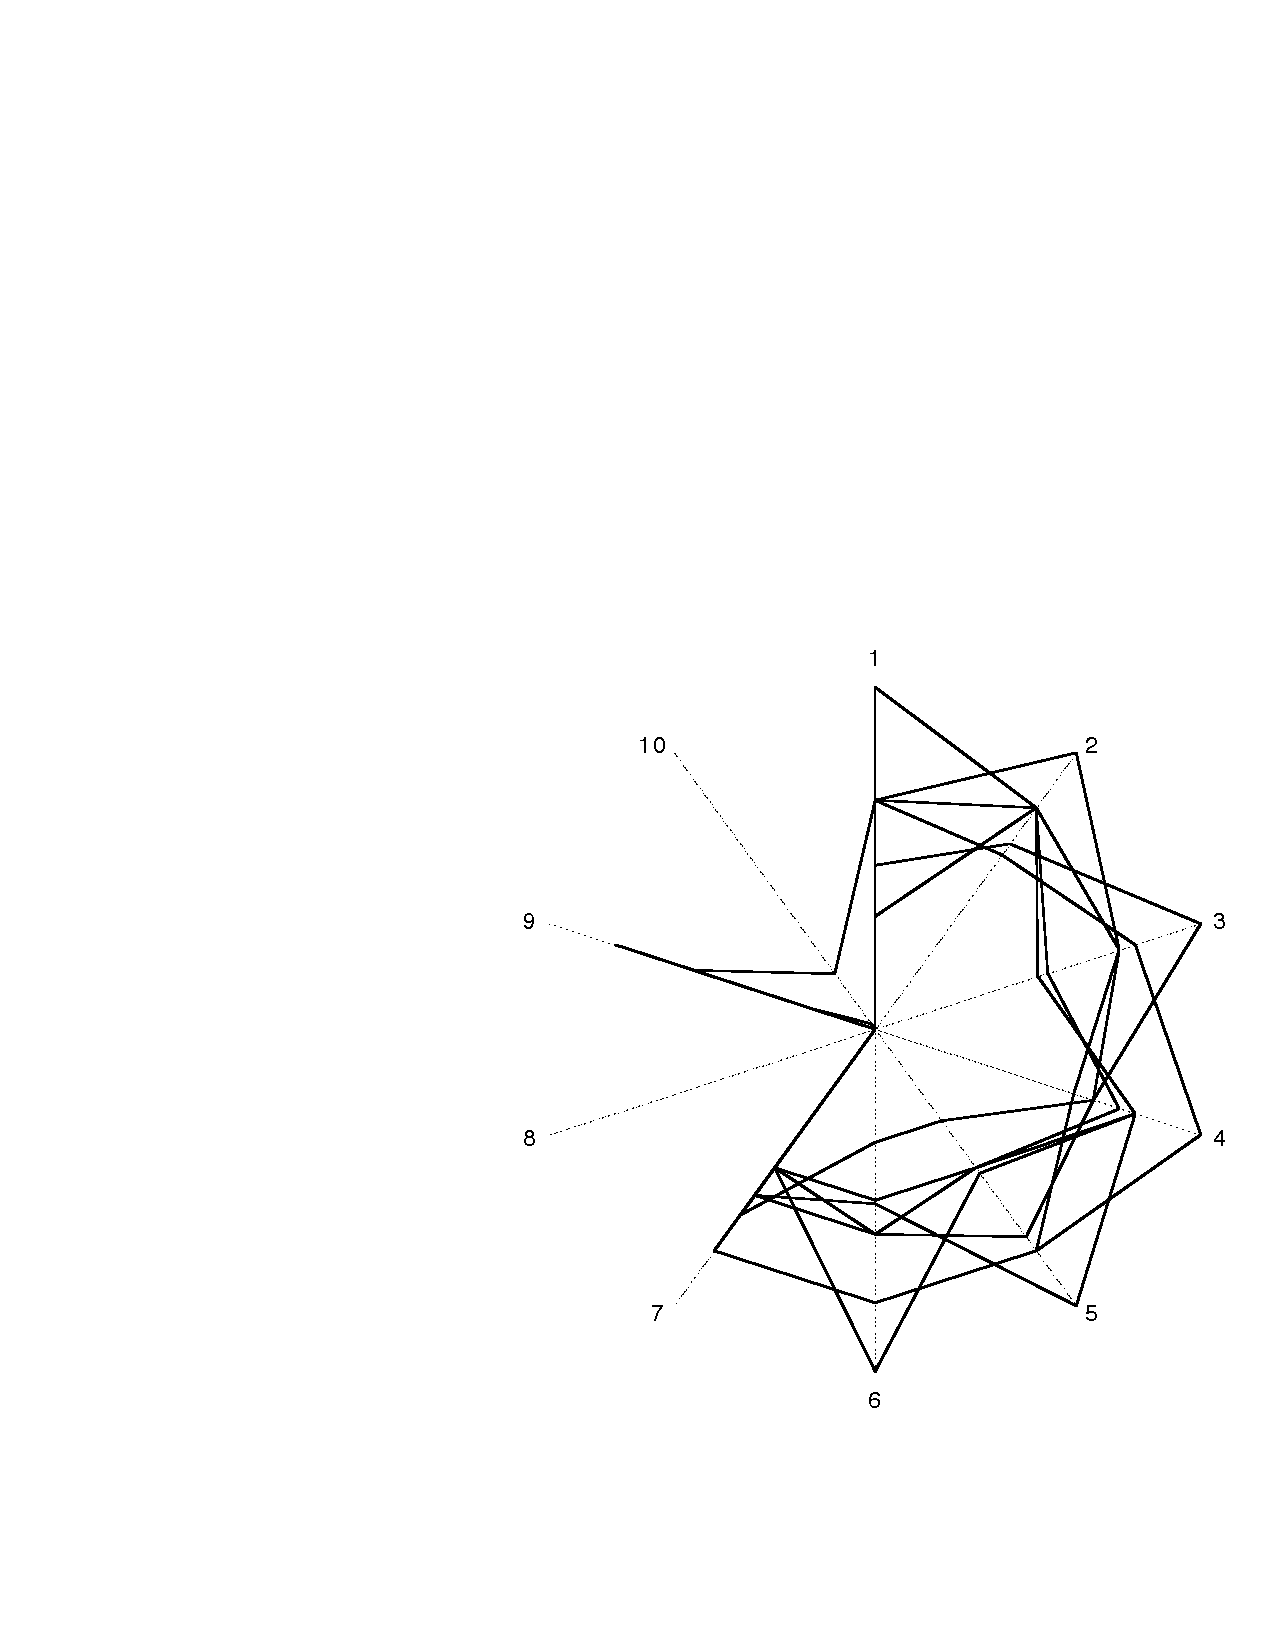
\includegraphics[width=.32\textwidth]{chap7/figs/com-4.pdf}
}
\centerline{
 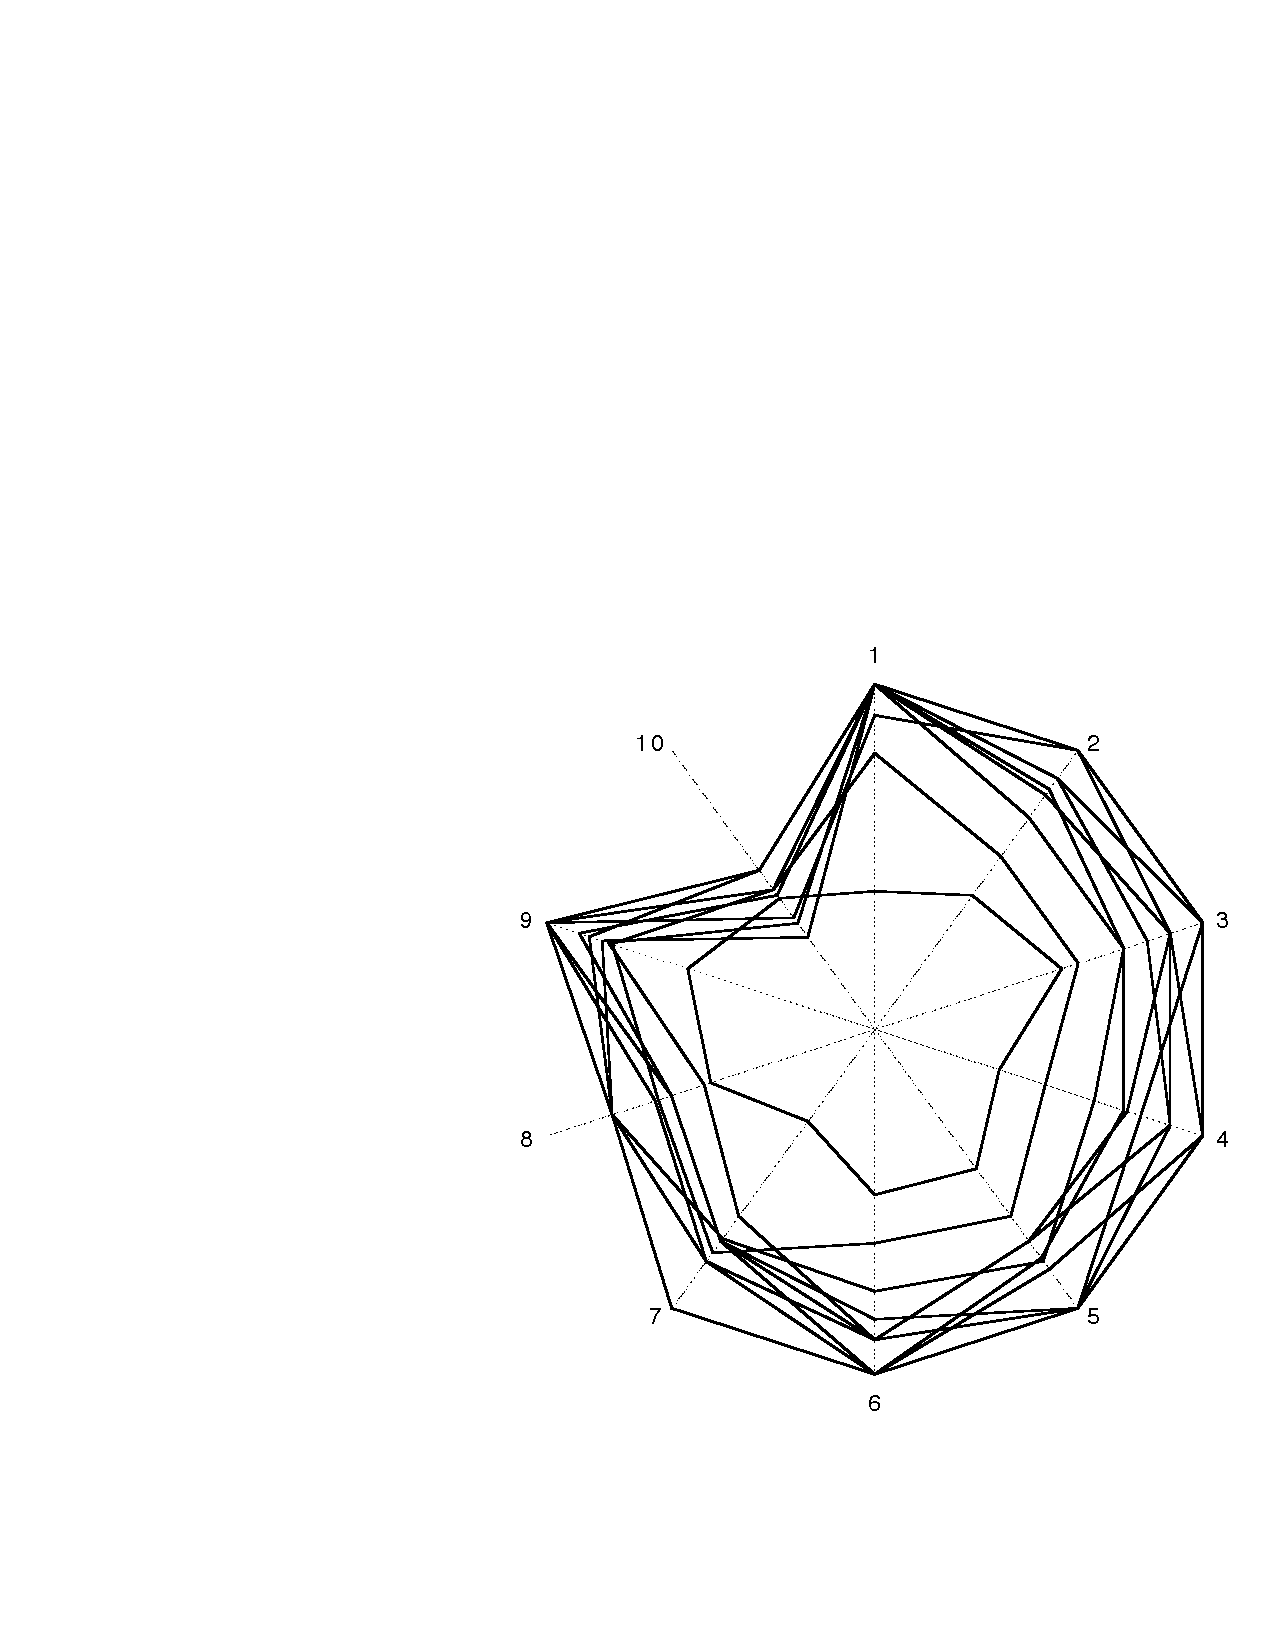
\includegraphics[width=.32\textwidth]{chap7/figs/com-6.pdf}
 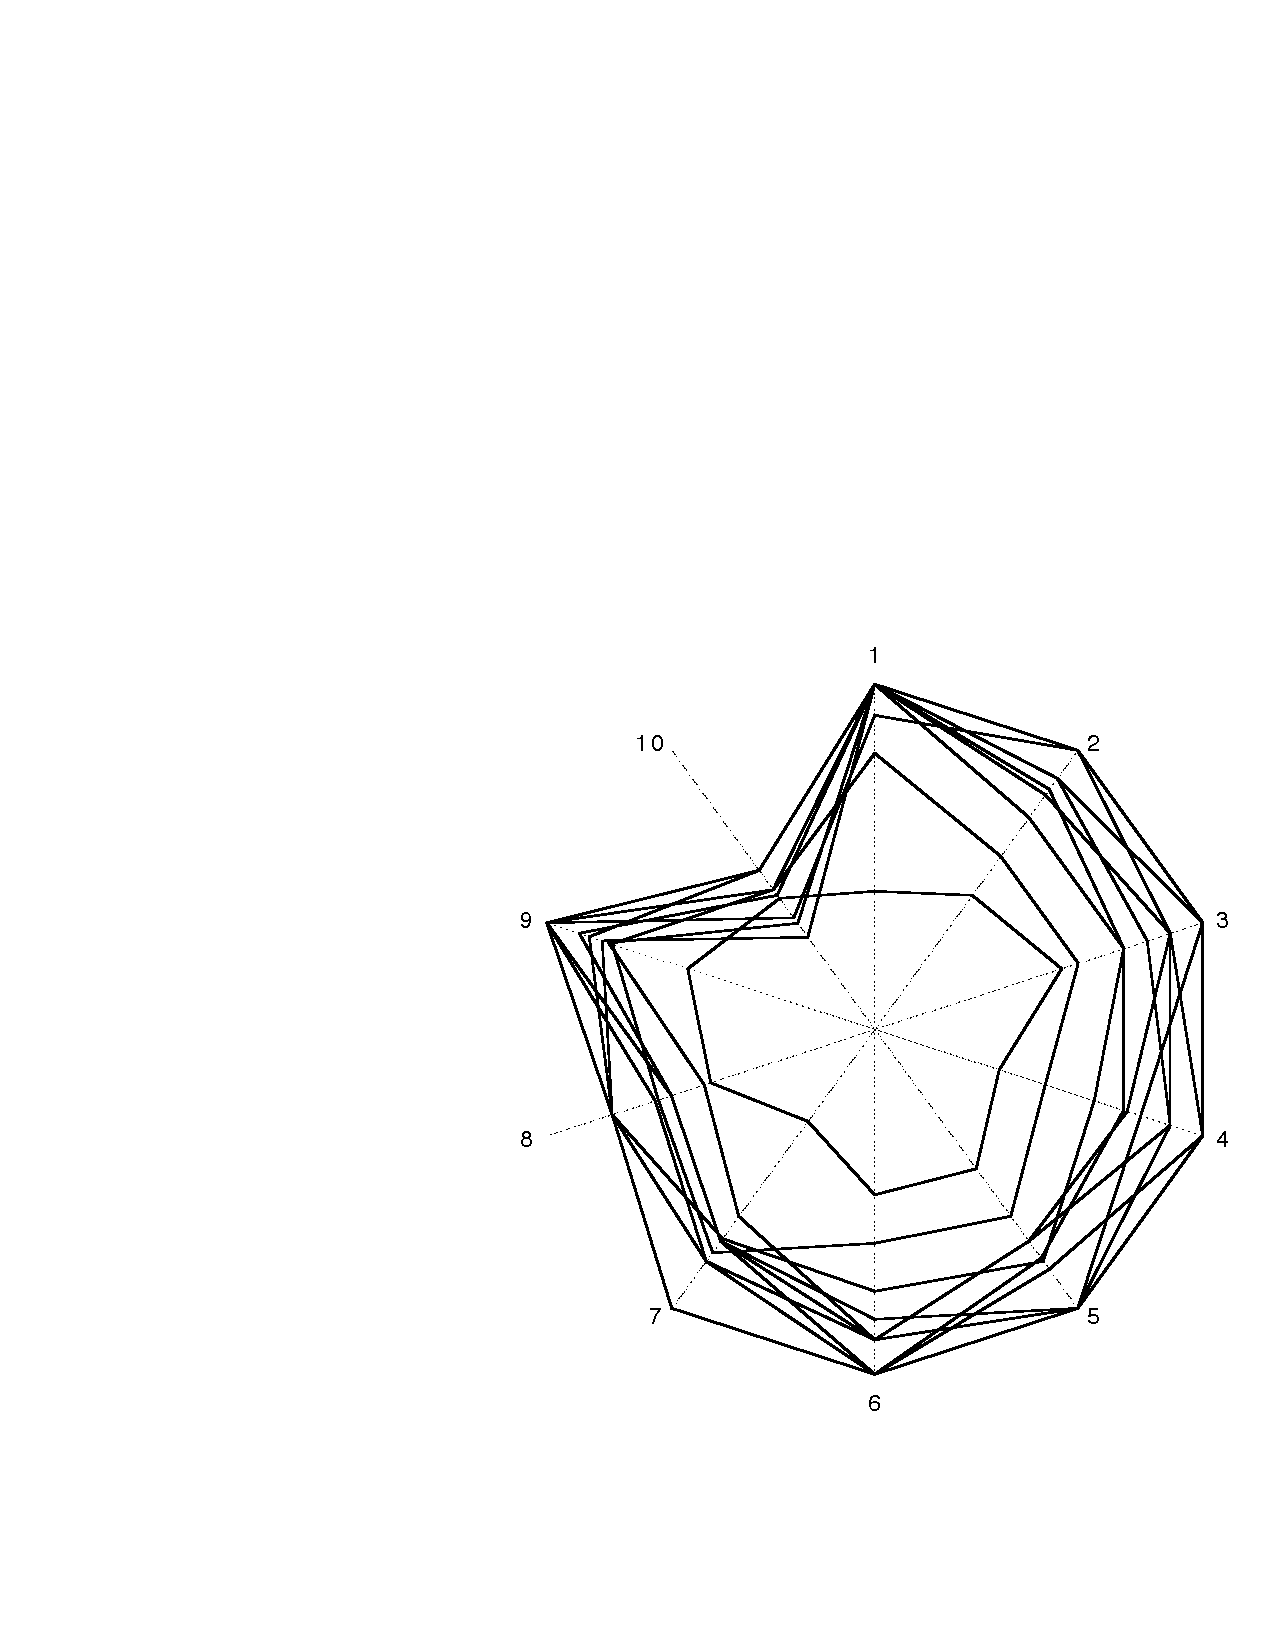
\includegraphics[width=.32\textwidth]{chap7/figs/com-8.pdf}
 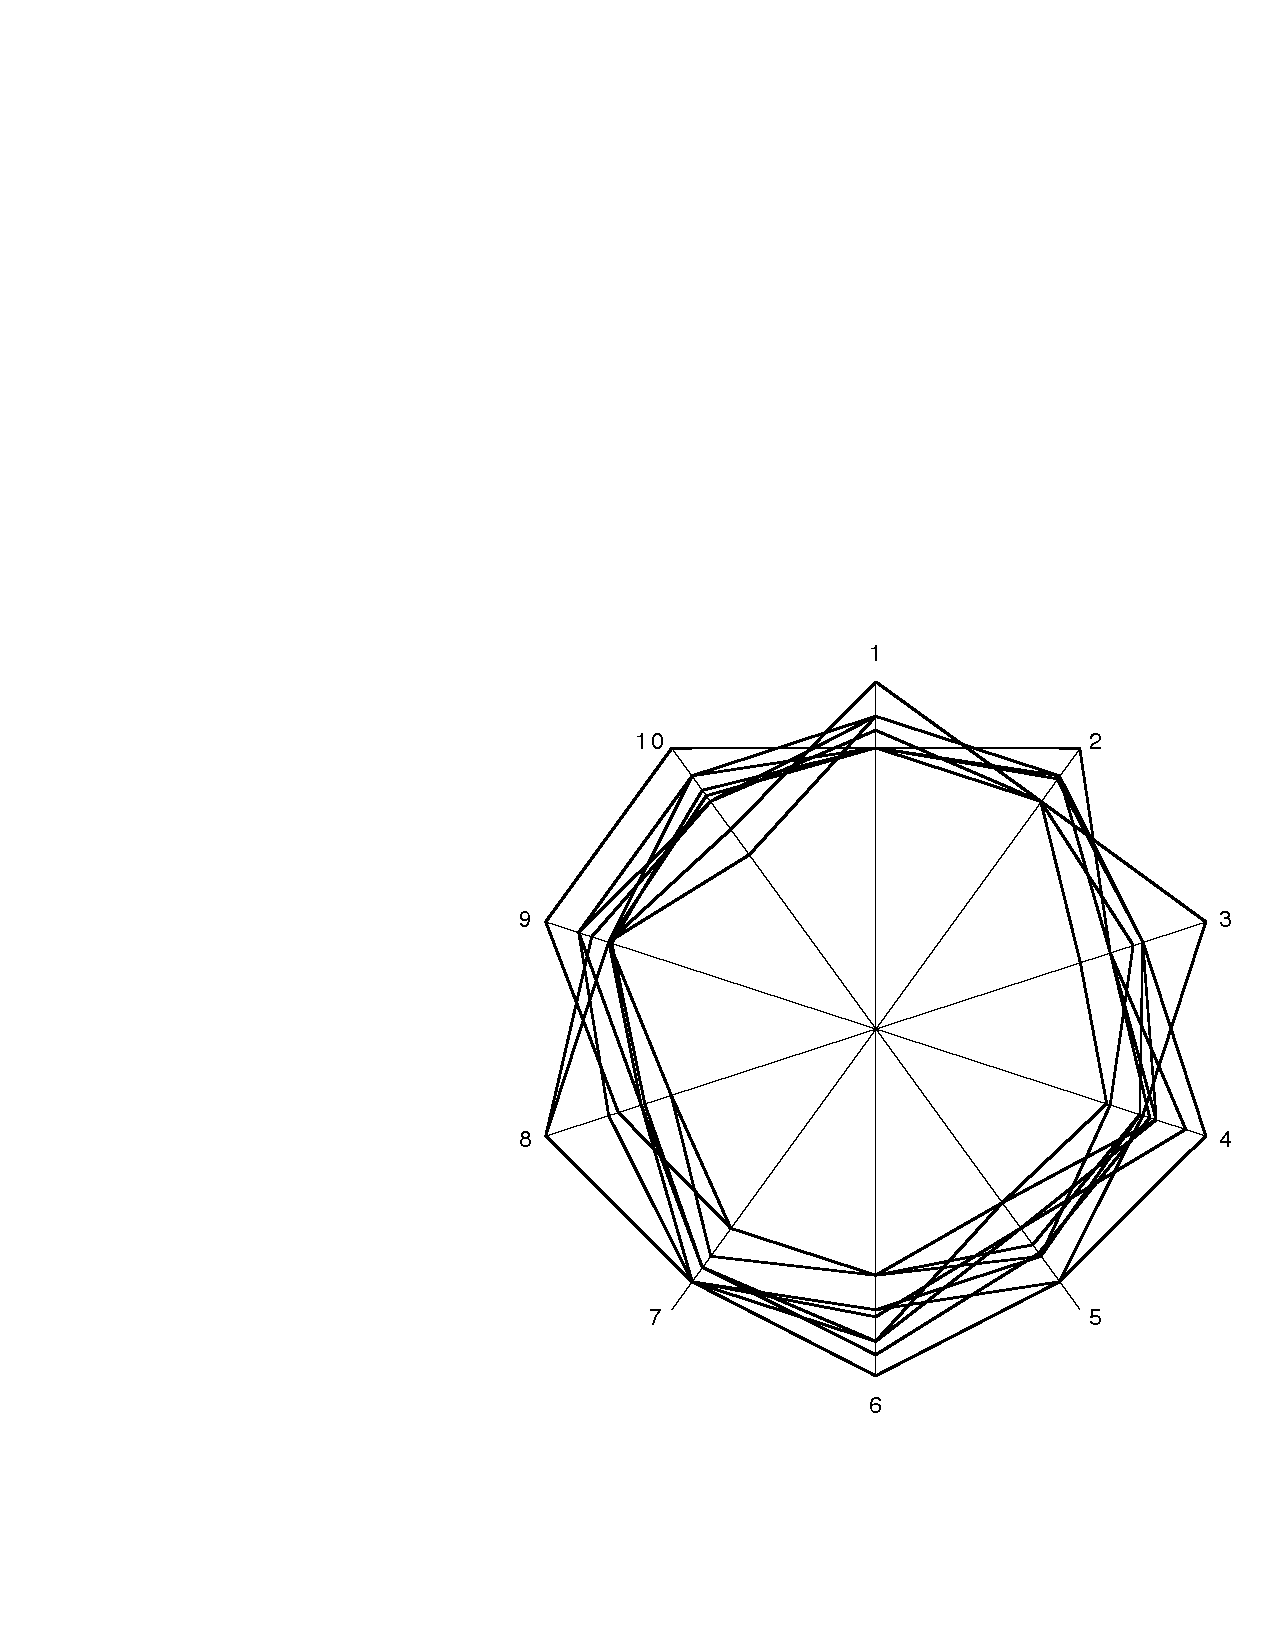
\includegraphics[width=.32\textwidth]{chap7/figs/com10.pdf}
}

\caption{\label{cohweb}Coherence diagrams visualising
the coherence of ontologies in a group of 10 agents for
a series of 1000 discrimination games. Lines emanate 
from the center when there is close to 0 \% coherence. They approach the
edges in the case of 100 \% ontological coherence.}
\end{figure}

